\chapter{Description of Three - Dimensional Elasticity}\label{chap1}

THIS\pageoriginale  CHAPTER WILL be divided into four sections. In the
first section 
some preliminaries on deformations in $\mathbb{R}^3$ will be
discussed; the second will be devoted to the equations of eqilibrium
and the third to constitutive equations. These together will give rise
to the boundary value problem which will serve as the model for three
- dimensional elasticity. The last section will describe the energy
functional and the associated Euler equations will be seen to give the
equations of equilinrium and the constitutive equations. 

\section{Geometrical Preliminaries}\label{chap1-sec1.1} %SEction 1.1

Let $\Omega \subset \mathbb{R}^3$ be a bounded open set. Let
$\mathfrak{B}_R = \bar{\Omega}$, the closure of $\Omega$ in
$\mathbb{R}^3$, stand for the \textit{reference configuration}.\index{reference configuration} (The
subsript $R$ will always stand for the reference configuration.) Let
$X_R$ be a generic point in $\mathfrak{B}_R$. If $\{e_1, e_2, e_3 \}$
is the standard orthonormal basis for $\mathbb{R}^3$,  
\begin{equation*}
OX_R = X_{R_i} e_i \tag{1.1-1}\label{eq1.1-1}
\end{equation*}
where\pageoriginale  $OX_R$ stands for the position vector of
$X_R$. (In the above 
relation and in all that follows, the summation convention for
repeated indices will always be adopted.) 

\begin{figure}[H]
\centering
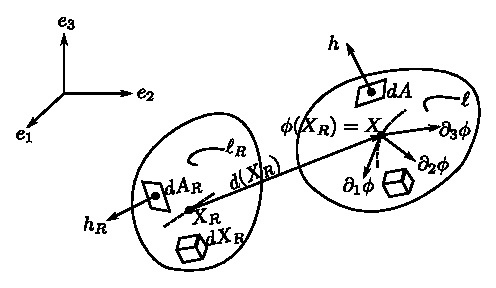
\includegraphics{vol71-figures/fig1.1-1.eps}
\medskip
\caption{}\label{fig1.1.1}
\end{figure}


Let $\phi : \mathfrak{B}_R \rightarrow \mathbb{R}^3$ be a
sufficiently regular mapping. It is said to be a \textit{deformation}
if  
\begin{equation*}
\det (\nabla  \phi ) > 0 \tag{1.1-2}\label{eq1.1-2}
\end{equation*}
where $\nabla  \phi$ is called the \textit{deformation\index{deformation}
 gradient}\index{deformation gradient} and is a matrix given by 
$$
\nabla  \phi
\begin{vmatrix}
\dfrac{\partial \phi_1} {\partial X_{R_1}}& \dfrac{\partial \phi_1}
    {\partial X_{R_2}} & \dfrac{\partial \phi_1} {\partial X_{R_3}}\\ 
      \dfrac{\partial \phi_2} {\partial X_{R_1}} & \dfrac{\partial
        \phi_2} {\partial X_{R_2}} & \dfrac{\partial \phi_2}
            {\partial X_{R_3}} \\ 
       \dfrac{\partial \phi_3} {\partial X_{R_1}} & \dfrac{\partial
         \phi_3} {\partial X_{R_2}} &  \dfrac{\partial \phi_3}
             {\partial X_{R_3}} \\ 
\end{vmatrix}
$$
$\phi_i$ being the components of $\phi$.
\begin{remark}\label{chap1:rem1.1.1} %Remark 1.1-1
From\pageoriginale  \eqref{eq1.1-2} it follows that $\phi$ is locally one -
one, though it 
may not be globally so. 
\end{remark}

The image set $\mathfrak{B} = \phi (\mathfrak{B}_R)$ is called the
\textit{deformed configuration}.\index{deformed configuration} Note that the mapping $\phi$ can be
written as 
\begin{equation*}
\phi = Id + u \tag{1.1-3}\label{eq1.1-3}
\end{equation*}
and the mapping $u : \mathfrak{B}_R \to \mathbb{R}^3$ is called the
\textit{displacment}.\index{displacement} It is also seen that 
\begin{equation*}
\nabla  \phi = I + \nabla  u \tag{1.1-4}\label{eq1.1-4}
\end{equation*} 
where $I$ is the identity matrix and $\nabla  u$ is the
\textit{displacement gradient}.\index{displacement gradient}  

The deformation gradient defines the deformation at $X = \phi (X_R)$
up to first order. If $ dt~ e_1$ is a line segment parallel to $e_1$
at $X_R$, it is transformed into a curve at $X$ whose tangent is $ dt
~\partial_1 \phi$, where $\partial_1 \phi$ is the first colums vector
of $\nabla  \phi$. The magnitude dt is now `streched' by dt
$|\partial_1 \phi|$, where $|.|$ stands for the Euclidean norm. The
three vectors $\partial_1 \phi$, $\partial_2 \phi$, $\partial_3 \phi$ are
independent and, owing to the relation \eqref{eq1.1-2}, preserve the
orientation of $\{e_1, e_2, e_3 \}$. 

It will now be seen how volume, area and line elements are transformed
under the defomation $\phi$. 
\begin{enumerate}[(i)]
\item \textit{Volume elements:} The change from a volume element
 $dX_R$ to $dX$ in the deformed confirguration comes from the
 familiar change of variable formula in interation theory: 
\begin{equation*}
 dx = \det (\nabla  \phi (X_R)) dX_R. \tag{1.1-5}\label{eq1.1-5}
\end{equation*}

\item \textit{Surface elements:} If $dA_R$ is a surface element on
 $\mathscr{B}_R$ deformed onto a surface elemment $dA$ on
 $\mathfrak{B}$, then 
\begin{equation*}
  dA = \det (\nabla  \phi (X_R)) | (\nabla  \phi
  (X_R))^{-t} n_R | dA_R \tag{1.1-6} \label{eq1.1-6}
\end{equation*}\pageoriginale 
where $n_R$ is the unit outer normal. (If $F$ is any matrix, $F^T$
stands for its transpose, $F^{-1}$ for its inverse and $F^{-T} =
(F^{-1})^T$). 

The formula \eqref{eq1.1-6} will now be proved . This needs some
preliminaries. Let $\mathbb{M}^3$ stand for the set of all $3 \times
3$ matrices. A tensor will be understood simply to be an element of
$\mathbb{M}^3$.  
\end{enumerate}

Let $T : \mathfrak{B} \to \mathbb{M}^3$ be a tensor field. Then
its \textit{divergence}\index{divergence of a tensor} (assuming $T$ to be smooth snough) is defined
by 
\begin{equation*}
  DIV T = \frac{\partial T_{ij}}{\partial X_j}
  e_i. \tag{1.1-7}\label{eq1.1-7} 
\end{equation*}

Thus each component of $DIV ~ T$ is the divergence (in the usual
sence) of the corresponding \textit{row} vector of $T$. By a standard
application of Green's formula it follows that 
\begin{equation*}
  \int \limits_\mathfrak{B} DIV T dX = \left(\int\limits_\mathfrak{B}
  \frac{\partial T_{ij}}{\partial X_j} dX \right) e_i = \left( \int
  \limits_\mathfrak{\partial B} T_{ij} n_j dA \right) e_j = \int \limits_{\partial
    \mathfrak{B}} T_n dA \tag{1.1-8} \label{eq1.1-8}
\end{equation*}
where $n$ is the units outer normal to $\mathfrak{B}$. In the same
vein $DIV_R (T_R)$ on tensor fields on $\mathfrak{B}_R$ can be defined
and the analogue of \eqref{eq1.1-8} can be obtained. 


Let $T : \mathfrak{B} \to \mathbb{M}^3$ be a tensor
field. Its\textit{Piola Transform}\index{Piola transform} is a tensor field $T _R:
\mathfrak{B}_R \to \mathbb{M}^3$ given by  
\begin{equation*}
  T_R(X_R) = \det (\nabla  \phi (X_R)) T(X) (\nabla
  \phi (X_R))^{-T} \tag{1.1-9} \label{eq1.1-9}
\end{equation*}
were $X = \phi (X_R)$.

This is a very useful transformation. The following theorem will
establish the formula \eqref{eq1.1-6}. 
\begin{theorem}\label{chap1-thm1.1.1} % 1.1-1
\begin{enumerate}[(i)]
\item $T_R (X_R) n_R dA_R = T(X) n dA$\pageoriginale 
\item $\det (V \phi (X_R)) (V \phi (X_R))^{-T} n_R dA_R = ndA$
\item $\det (\nabla \phi (X_R)) | (\nabla  \phi
 (X_R))^{-T} n_R | dA_R = dA$. 
\end{enumerate}
\end{theorem}

\begin{proof}
It can be shown that (cf. Exercise 1.1-1).
\end{proof}
\begin{equation*}
DIV_R T_R (X_R) = \det (V \phi (X_R)) DIV T(X) \tag{1.1-10}\label{eq1.1-10}
\end{equation*}

If $v_R$ is any arbitrary volume in $\mathfrak{B}_R$ and
$\vartheta = \phi (v_R)$, then 
\begin{align*}
\int \limits_{\partial v_R} T_R (X_R) n_R dA_R & = \int
\limits_{\partial v_R} DIV_R T_R (X_R) dX_R \\ 
& = \int \limits_{v_R} \det (\nabla
\phi(X_R)) DIV T(X_R)) dX_R \\ 
& = \int \limits_{v_R} DIV T(X) dX = \int
\limits_{\partial v} T(X) n dA 
\end{align*}
which, as $v$ was arbritrary, proves (i). The assertion
(ii) follows by setting $T = I$. This is a vector relation and
taking the Euclidean norm on both sides gives (iii). 

\begin{remark}\label{chap1-rem1.1-2} %Remark 1.1-2
  The matrix $\det (\nabla \phi) (\nabla  \phi)^{-T} =
  (\adj  \nabla \phi)^{-T}$ is the matrix of cofactors of
  $\nabla  \phi$. 
\end{remark}
(iii) Line elements: If $\phi$ is smooth enough, 
$\phi (X_R + \delta X_R ) - \phi(X_R) = \nabla  \phi (X_R)
\delta X_R + o (\delta X_R)$. 

Thus
\begin{equation*}
| \phi (X_R + \delta X_R ) - \phi (X_R) |^2 = \delta X^T_R
\nabla  \phi (X_R)^T \nabla  \phi (X_R) \delta X_R +
o(|\delta X_R|^2) \tag{1.1-11} \label{eq1.1-11}
\end{equation*}
which gives the change in length. The matrix 
\begin{equation*}
C = \nabla  \phi^T \nabla  \phi \tag{1.1-12}\label{eq1.1-12}
\end{equation*}
is\pageoriginale  called the  \textit{(right) Cauchy - Green strain
  tensor} and will 
play an important role in the theory. It is used to compute the length
of an arc. If $f(I)$ is a curve $\ell_R$ in $\mathfrak{B}_R$, where $I
\subset \mathbb{R}$ is an interval, and $\ell = \phi (\ell_R)$ is its
image in $\mathfrak{B}$, then the length of $\ell$ is given by 
$$
\int \limits_I | (\phi of)' (t) | dt = \int \limits_I \sqrt{c_{ij}
 (f(t)) f'_i(t) f'_j (t)} dt 
$$
where $C_{ij}$ are the components of the matrix $C$ defined above.

\begin{remark}\label{chap1-rem1.1.3} %Remark 1.1-3
The matrix
\begin{equation*}
 B = \nabla  \phi \nabla \phi^T \tag{1.1-13}\label{eq1.1-13}
\end{equation*}
called the \textit{(left) Cauchy-Green strain
  tensor}\index{Cauchy-Green strain tensors}\index{strain!CAUCHY-GREEN-tensors} will be 
introduced later and will play an important role in the constitutive
equations. 
\end{remark}

\begin{remark}\label{chap1-rem1.1.4} %Remark 1.1-4
The change in volume depends on a scalar $\det \nabla
\phi$. The change is surface elements depends on a matrix, ($\adj
\nabla \phi$) and the change in line elements on a matrix, $C
= \nabla  \phi^T \nabla  \phi$. All these will figure
in the integral representing the energy (cf. Sect. \ref{chap2-sec2.6}). 
\end{remark}

To conclude this section, it will now be examined to what extent the
strain tensor $C$ is a measure of the deformation. The word
`deformation' can be interpreted in two ways - first the formal sense
as defined earlier in this section; secondly, in an intuitive way
which can be described as follows. If $\phi$ were merely to consist of
a translation and then a rotation about a point in space, while it is
a deformation in the strict sense, yet distances between points are
not altered. So intuitively the body has not been `deformed', Such a
transformation is called a rigid deformation. 

Thus, $\phi$ is said to be a \textit{rigid deformation}\index{rigid deformation} if 
\begin{equation*}
\phi{(X_R)} = a + Q (OX_R),\tag{1.1-14}\label{eq1.1-14} 
\end{equation*}\pageoriginale 
where a $\in \mathbb{R}^3$ and $Q$ is an orthogonal matrix whose
determinant is $ + 1$. 

The vector a above represents a translation and the matrix $Q$ a
rotation. The following notation will used for various classes of
matrices: 
\begin{align*}
\mathbb{M}^3_+ & = \{F \in \mathbb{M}^3 | \det (F) > 0 \} \\
\mathbb{O}^3 & = \{F \in \mathbb{M}^3 | F^T F = FF^T = I \} \\
 \mathbb{O}^3_+ & = \{F \in \mathbb{O}^3 | \det (F) = + 1 \} \\
 \mathbb{S}^3 & =\{F \in \mathbb{M}^3 | F^T = F \} \\
 \mathbb{S}^3_> & =\{F \in \mathbb{S}^3 | F \text {is positive definite}\}. 
\end{align*}

Thus $Q \in \mathbb{O}^3_+$ . Observe that if $\phi$ is rigid then $C
= Q^T Q = I$. In fact, under suitable hypotheses, the converse is also
true. 

\begin{theorem}\label{chap1-thm1.1.2} %Theorem 1.1-2
	Let $\Omega$ be an open connected subset of
          $\mathbb{R}^3$. Let $\phi \in C^1 (\Omega ; \mathbb{R}^3 )$
          such that for all $x \in \Omega$, 
\begin{equation*}
\nabla  \phi (x)^T \nabla  \phi (x) = I \tag{1.1-15}\label{eq1.1-15}
\end{equation*}

Then, there exists a vector $a \in \mathbb{R}^3$ and a matrix
 $Q \in \mathbb{O}^3$ such that, for all $x \in \Omega$
\begin{equation*}
\phi (x) = a + Q(0x). \tag{1.1-16}\label{eq1.1-16}
\end{equation*}
\end{theorem}

\begin{proof}
Cf. Exercise 1.1-2
\end{proof}

\begin{theorem}\label{chap1-thm1.1.3} %Theorem1.1-3
Let $\Omega$ be an open connected subset of $\mathbb{R}^3$ and let
$\phi, \psi \in C^1 (\Omega ; \mathbb{R}^3$) such that for all $x \in
\Omega$ 
\begin{equation*}
\nabla  \phi (x)^T \nabla  \psi (x) = \nabla
\psi (x)^T \nabla  \phi (x). \tag{1.1-17} \label{eq1.1-17}
\end{equation*}

 Assume\pageoriginale  further that $\psi$ is one - one and that $\det (\nabla
 \psi(x)) \neq 0$ for all $x \in \Omega$. Then there exists $a \in
 \mathbb{R}^3$ and $Q \in O^3$ such that for all $x \in \Omega$ 
\begin{equation*}
\phi (x) = a + Q \psi (x). \tag{1.1-18}\label{eq1.1-18}
\end{equation*}
\end{theorem}

\begin{proof}
Consider the mapping $\theta = \phi o \psi^{-1}$ on
$\psi(\Omega)$. Clearly $\psi (\Omega)$ is connected. Also, under the
given conditions, it is open by the theorem of invariance of
domain. Further, $\theta \in C^1 (\psi (\Omega); \mathbb{R}^3$). Now
from \eqref{eq1.1-17} it follows that $\theta$ satisfies
\eqref{eq1.1-15} and so the previous theorem applies to $\theta$ and
the result follows.  
\end{proof}

Thus if two deformations have the same strain tensor then, upto a
rigid deformation, they are the same. Thus $C$ `measures' the
`deformation' upto a rigid transformation. Naturally, a measure of the
deviation from a rigid deformation is obtained from $C -
I$. \textit{The Green-St Venant strain tensor},\index{Green-St Venant
  strain tensor}\index{strain!Green-St Venant-tensor}  $E$, is defined by the relation 
\begin{equation*}
C - I = 2 E \tag{1.1-19}\label{eq1.1-19}
\end{equation*}

In terms of the displacement gradient, 
$$
I + 2 E = C = \nabla  \phi^T \nabla  \phi = I +
\nabla u^T + \nabla u + \nabla u^T
\nabla u 
$$
or, componentwise, 
\begin{equation*}
E_{ij} = \frac{1}{2}(\partial _i u_j + \partial_j u_i + \partial_i u_m
\partial_j u_m) \tag{1.1-20} \label{eq1.1-20}
\end{equation*}
where $\partial_i$ stands for $\dfrac{\partial}{\partial X_{R_i}}$

\medskip
\begin{center}
{\large\bf{Exercises}}
\end{center}

\begin{description}
\item[1.1-1] Prove\pageoriginale  the \textit{Piola identity}\index{Piola identity}
$$
DIV_R (det (\nabla  \phi (X_R)) (\nabla  \phi((X_R))^{-T}) = 0.
$$

Deduce the relation \eqref{eq1.1-10} from this.

\item[1.1-2.] Prove Theorem \ref{chap1-thm1.1.2} (Hint: First show
  that at least 
locally, $\phi$ is an isometry; then show $\nabla  \phi$ is
locally contant and use the connectendness of $\Omega$.) 
 
\item[1.1-3.] Let $\phi : \mathbb{R}^n \to \mathbb{R}^n , n \geq 2, $
 be continuous. Assume that there exists $\ell > 0$ such that for all
 $x, y \in \mathbb{R}^n$ with $|x - y| = \ell , |\phi (x) - \phi (y)|
 = \ell$. Show that $\phi$ is an isometry, i.e. there exists $a \in
 \mathbb{R}^n$ and $Q \in \mathbb{O}^n$ such that for all $x \in 
 \mathbb{R}^n$ 
 $$
 \phi (x) = a + Qx.
 $$

\item[1.1-4.] Given a tensor field $\Gamma : \Omega \to
 \mathbb{S}^3$, find necessary and sufficient conditions such that
 there exists a mapping $\phi : \Omega \to \mathbb{R}^n$ with 
 $$
 \Gamma = \nabla  \phi^T \nabla  \phi 
 $$
\end{description}

\section{Euilibrium Equations}\label{chap1-sec1.2}
\setcounter{figure}{0} 

The equilibrium equations give the relationship between the given
forces acting on a body and the state of ``stress" (to be defined
below) which results as a consequence of these forces. 
 
Let the mass density as $X \in \mathfrak{B}$ be given by $\rho(X)$
while that at $X_R \in \mathfrak{B}_R$ is given by $\rho_R (X_R)$. The
applied forces in $\mathfrak{B}$ are of two kinds. 


\begin{figure}[H]
\centering
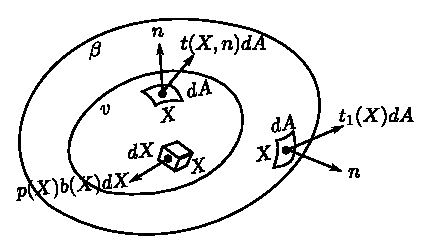
\includegraphics{vol71-figures/fig1.2-1.eps}
\medskip
\caption{}\label{fig1.2.1}
\end{figure}\pageoriginale 

\begin{enumerate}[(i)]
\item \textit{Body ({\em or} volumic) forces:}\index{force: applied surface!body} $b: \mathfrak{B} \to
  \mathbb{R}^3$. The elementary force on a volume element $dX$ will
  thus be $\rho(X) b(X) dX$. An example of a body force\index{body
    force} is gravity 
  and in this case $b = (o, o, -g)$. 

\item \textit{Applied surface forces:}\index{applied surface
  force}\index{force: applied surface}\index{force: applied surface!surface}
  $t_1 : \partial \mathfrak{B}_1 
  \rightarrow \mathbb{R}^3$, where $\partial \mathfrak{B}_1$ is a
  portion of the boundary $\partial \mathfrak{B}$. If $dA$ is a
  surface element, the applied force on it will be $t_1 dA$. An
  example of a surface force\index{surface force} is a pressure load where $t_1 = -pn, p
  \in \mathbb{R}, n$ the normal to $dA$. 
\end{enumerate} 

A \textit{system of forces}\index{force: applied surface!system of}\index{system of forces} in $\mathfrak{B}$ consists of \textit{body
  forces} (identical to (i) above) and \textit{surface forces} $t:
\mathfrak{B} \times \Sigma_1 \to \mathbb{R}^3$ where $\Sigma_1$ is the
unit sphere in $\mathbb{R}^3$, i.e.,  
$$
\Sigma_1 = \{x \in \mathbb{R}^3 || x | = 1 \}.
$$

If $\vartheta$ is any subvolume of $\mathfrak{B} , dA$ a surface
element of $\partial \vartheta$ and $n$ the normal to it, the surface
force $t (X, n) dA $ acts in it. Note that this is independent of
$\vartheta$, i.e. if $\vartheta_1$ were another subvolume and $dA$
lay on $\partial v_1$ with the same $n$ as normal, the force acting on
it  will\pageoriginale  remain as $t(X,n)dA$. Further if $dA \subset \partial
\mathfrak{B}$ and $n$ were also normal to $\partial \mathfrak{B}$, it
is required that 
\begin{equation*}
t(X,n) = t_1 (X).\tag{1.2-1}\label{eq1.2-1}
\end{equation*}

The vector $t(X,n)$ is called the \textit{Cauchy stress
  vector}.\index{Cauchy stress vector}\index{stress!CAUCHY - vector} 

The following axiom is the basis of Continuum Mechanics in general,
and consequently of the theory of elasticity in particular. 

\medskip
\textit{AXIOM OF STATIC EQUILIBRIUM.\index{axiom of static
    equilibrium} Let $\mathfrak{B}$ be a deformed 
configuration in static equilibrium. There exists a system of forces
such that for any subdomain $\vartheta \subset \mathfrak{B}$,the
corresponding system of forces is equivalent to zero (in the sense of
torsors). Thus} 
\begin{align*}
  \int\limits_\vartheta ~\rho(X)~ b(X) ~dX~ +
  ~\int\limits_{\partial\vartheta}~ t(X,n)~ dA &= o.\tag{1.2-2}\label{eq1.2-2} \\
  \int\limits_{\vartheta} OX \Lambda \rho(X) b(X) dX +
  \int\limits_{\partial\vartheta} OX \Lambda t(x,n) dA & =
  o.\tag{1.2-3} \label{eq1.2-3} 
\end{align*}

The wedge $\Lambda$ stands for the usual cross product of vectors in
$\mathbb{R}^3$. The following notation will be useful in manipulating
cross products. 

For indices $i$, $j$, $k$ taking values 1, 2, 3 the tensor of rank
$3,\epsilon_{ijk}$, is defined by 
\begin{equation*}
  \epsilon_{ijk}=
  \begin{cases}
    +1 & \text{if} (i,j,k) \text{is an even permutation of} (1,2,3),\\
    -1 & \text{if it is an odd permutation of} (1,2,3),\\
    0 & \text{otherwise}.
  \end{cases}
  \tag{1.2-4}\label{eq1.2-4}
\end{equation*}

Then for vector $a,b \epsilon \mathbb{R}^3$,
\begin{equation*}
  a \Lambda b = \epsilon_{ijk} a_j b_k e_i.\tag{1.2-5}\label{eq1.2-5}
\end{equation*}

The\pageoriginale  following consequence of the axiom of static
equilibrium is of paramount importance. 

\begin{theorem}[Cauchy's Theorem]\label{chap1-thm1.2.1}%THEOREM 1.2-1
Let\index{Cauchy's Theorem} $\rho \epsilon C^\circ(\mathfrak{B}$ ;
  $\mathbb{R})$, $b \epsilon C^\circ(\mathfrak{B}$;$\mathbb{R}^3)$,
  $t(.,n)$ $\epsilon C^1(\mathfrak{B}; \mathbb{R}^3)$ and
  $t(X,.)\epsilon C^\circ (\sum_1 ; \mathbb{R}^3)$. Then there
  exists a tensor field $T \epsilon C^1$ $(\mathfrak{B}$;
  $\mathbb{M}^3)$ such that 
\begin{align*}
  t(X,n) & = T(X) n, ~\text{for all}~ X\epsilon
  \mathfrak{B},n\epsilon \Sigma_1,\tag{1.2-6} \label{eq1.2-6}\\ 
  DIV T(X) + \rho(X)~ b(X) & = 0, ~\text{for all}~ X \epsilon
  \mathfrak{B},\tag{1.2-7}\label{eq1.2-7}\\ 
  T(X) &= T^T(X), ~\text{for all}~ X \epsilon
  \mathfrak{B}.\tag{1.2-8} \label{eq1.2-8}
\end{align*}
\end{theorem}

\begin{proof}
Let $X_0$ be any point in $\mathfrak{B}$. Consider a tetrahedron
$\vartheta$ with vertices $X_0,V_1,V_2,V_3$ as shown in
Fig.~\ref{fig1.2.2}.  
\end{proof}

\begin{figure}[H]
\centering
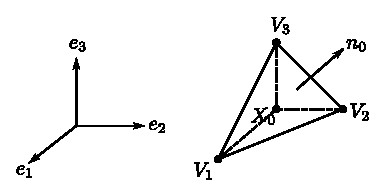
\includegraphics{vol71-figures/fig1.2-2.eps}
\caption{}\label{fig1.2.2}
\end{figure}

Let $n_0 \epsilon \sum_1$ be the normal to the plane $V_1 V_2 V_3$
and keep $n_\circ$ fixed to begin with. Let the distance of $X_\circ$
to the plane be $\delta$, let $S_i(i = 1,2,3)$ be the surface opposite
the vertex $V_i(i = 1,2,3)$ and $S$ the surface opposite $X_0$. Since
$\rho,b$ are continuous on $\mathfrak{B}$, they are bounded. Thus by
(\ref{fig1.2.2}), 
$$
| \int\limits_{\partial \vartheta}t(x,n) dA | \leq K Vol (\vartheta)
$$
$K$\pageoriginale  being a constant independent of $\delta$. Since Vol$(\vartheta) =
K_1 \delta^3$, $A(\delta)$ = Area of $S = K_2 \delta^2, K_1,K_2$ being
independent of $\delta$, it follows that  
\begin{equation*} 
\lim_{\delta \to O} \frac{1}{A(\delta )}
\int\limits_{\partial\vartheta}t(X,n)dA = 0\tag{1.2-9} \label{eq1.2-9}
\end{equation*}

Now,
$$
\lim_{\delta \rightarrow O} \frac{1}{A(\delta)}~\int\limits_S~
  t(X,n)~dA = t(X_O,n_O)
$$
and
$$
  \lim{\delta \rightarrow 0} \frac{1}{A(\delta)}\int\limits_{S_i} t(X,n)
  dA = (n_O.e_i) t(X_O,-e_i)
$$
using the continuity of the given functions. Hence by \eqref{eq1.2-9},
\begin{equation*}
t(X_\circ ,n_\circ) = - (n_\circ . e_i) t(X_\circ ,-e_\circ
).\tag{1.2-10}\label{eq1.2-10} 
\end{equation*}

If $n_\circ \to e_j$, again by continuity of $t$ it follows that 
$$
t(X_\circ ,e_j) = - t(X_\circ,-e_j).
$$

Thus, on substituting this in \eqref{eq1.2-10},
\begin{equation*}
t(X_O,n_O) = t(X_O, e_j) n_j.\tag{1.2-11}\label{eq1.2-11}
\end{equation*}

Setting
$$
t(X_\circ ,e_j) = T_{ij} (X_\circ) e_i
$$
the equation \eqref{eq1.2-6} follows. The smoothness of $T$ results from
that of $t$ w.r.t. $X$. 

Using \eqref{eq1.2-6} in \eqref{eq1.2-2}, for any volume $\vartheta$,
\begin{align*}
0 & = \int\limits_{\vartheta} \rho (X) b(X) dX +
\int\limits_{\partial\vartheta} T(X) n dA\\ 
& = \int\limits_{\vartheta} \rho (X) b(X) + DIV (T) dX,
\end{align*}\pageoriginale 
from which \eqref{eq1.2-7} follows as $\vartheta$ was aribitrary.

Finally by \eqref{eq1.2-3} and \eqref{eq1.2-5}
\begin{align*}
0 & = \int\limits_L \epsilon_{ijk} X_j \rho(X)b_k(X) dX
+ \int\limits_{\partial\vartheta} \epsilon_{ijk} X_j T_{k\ell}
n_{\ell} dA\\ 
& = - \int\limits_{\vartheta} \epsilon_{ijk} X_j\frac{\partial
  T_{k \ell}}{\partial X_{\ell}} dX + \int\limits_{\partial\vartheta}
\epsilon_{ijk} X_j T_{k\ell} n_{\ell} dA\\ 
& = \int\limits_{\vartheta} \epsilon_{ijk} \frac{\partial
  X_j}{\partial X_\ell} T_{k\ell} dX = \int\limits_{\vartheta}
\epsilon_{i\ell k} T_{k\ell}, 
\end{align*}
using \eqref{eq1.2-7}. Since $\vartheta$ was arbitrary,
$$
\epsilon_{i\ell k} T_{k\ell} = 0
$$
which is just a restatement of \eqref{eq1.2-8}.

\begin{remark}\label{chap1-rem1.2.1}% Remark 1.2-1
  Given a tensor field $T : \mathfrak{B} \rightarrow \mathbb{M}^3$
  satisfying \eqref{eq1.2-7} and \eqref{eq1.2-8}, 
the vector field $t(X,n) = T(X)n$
  satisfies \eqref{eq1.2-2} and \eqref{eq1.2-3}. 
\end{remark}

The tensor $T(X)$ obtained in the above theorem is called the
\textit{Cauchy stress tensor}\index{Cauchy stress tensor}\index{stress!CAUCHY - tensor} at the point $X \epsilon
\mathfrak{B}$. 

\begin{figure}[H]
\centering
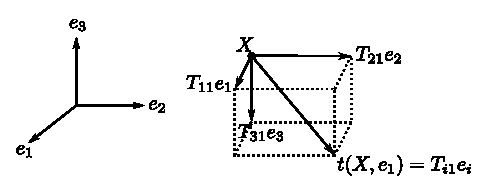
\includegraphics{vol71-figures/fig1.2-3.eps}
\caption{}\label{fig1.2.3}
\end{figure}

\begin{remark}\label{chap1-rem1.2.2}%Remark 1.2-2
The\pageoriginale  components of $T$ can be interpreted as follows. If
an element 
$dA$ has normal $e_1$ then the Cauchy stress vector\index{Cauchy
  stress vector}\index{stress!CAUCHY - vector}  acting on it, 
$t(X,e_1)$ has components $T_{11},T_{21}$ and $T_{31}$ and so on. 
\end{remark}

The Cauchy stress tensor thus satisfies a boundary value problem:
\begin{align*}
  \left.
  \begin{aligned}
    DIV T + \rho b & = 0\\
    T & = T^T
  \end{aligned}
  \right\}
  \text{in} ~\mathfrak{B}~\\
    T_n = t_1 ~\text{on}~ \partial\mathfrak{B}_1
\end{align*}

Let $u.v$ stand for the usual scalar product in $\mathbb{R}^3$,
i.e. $v.v = u_i v_i$. If $A,B \epsilon \mathbb{M}^3$, denote 
\begin{equation*}
A : B = A_{ij} B_{ij} = \tr (AB^T).\tag{1.2-12}\label{eq1.2-12}
\end{equation*}

This is an inner product in $\mathbb{M}^3$ with the associated norm
\begin{equation*}
\| A \| = \sqrt{A_{ij} A_{ij}}.\tag{1.2-13}\label{eq1.2-13}
\end{equation*}

Using Green's formula, a variational form of the boundary value
problem can be obtained. 

If $T$ is a tensor field and \textcircled{H} is a vector field on
$\mathfrak{B}$ then 
\begin{align*}
\int\limits_{\mathfrak{B}} DIV~T.\text{\textcircled{H}} dX & =
\int\limits_{\mathfrak{B}} \frac{\partial T_{ij}}{\partial X_j}
\text{\textcircled{H}}_i dX\\ 
& = -\int\limits_{\mathfrak{B}} T_{ij} \frac{\partial
  \text{\textcircled{H}}_i}{\partial X_j} dX + \int\limits_{\partial
  \mathfrak{B}} T_{ij} \text{\textcircled{H}}_i n_j dA\\ 
& = -\int\limits_{\mathfrak{B}} T : GRAD \text{\textcircled{H}} dX +
\int\limits_{\partial \mathfrak{B}} Tn.\text{\textcircled{H}} dA. 
\end{align*}

In\pageoriginale  particular, if $T$ is a solution of the above boundary value
problem and if \textcircled{H} vanishes on $\partial \mathfrak{B}_0 =
\partial \mathfrak{B}\backslash \partial \mathfrak{B}_1$, then Green's
formula above gives 
\begin{align*}
  0 & = \int\limits_{\mathfrak{B}} (DIV T + \rho b). \text{\textcircled{H}}dX\\
  & = \int\limits_{\mathfrak{B}} (-T: GRAD \text{\textcircled{H}} + \rho
  b. \text{\textcircled{H}} )dX + \int\limits_{\partial \mathfrak{B}_1}
  t_1.\text{\textcircled{H}}dA. 
\end{align*}

Conversely if the above relation is satisfied for all \textcircled{H}
vanishing on $\partial \mathfrak{B}_0$ then $T$ is a solution of the
boundary value problem. Thus  

\begin{theorem}\label{chap1-thm1.2.2}% Theorem 1.2-2
The following are equivalent:

\begin{itemize}
\item[\rm(i)] 
    $\begin{cases}
      DIV  T + \rho b &= 0, in \mathfrak{B}\\
      \quad Tn & = t_1  ~\text{in}~ \partial \mathfrak{B}_1
    \end{cases}$

\item[\rm (ii)] For all \textcircled{H} : $\mathfrak{B} \rightarrow
  \mathbb{R}^3$, \textcircled{H} vanishing on $\partial
  \mathfrak{B}_O$, 
  \begin{equation*}
    \int\limits_{\mathfrak{B}} T : GRAD \text{\textcircled{H}}dX = \int
    \rho b.\text{\textcircled{H}}dX + \int\limits_{\partial
      \mathfrak{B}_1} t_1.{\text{\textcircled{H}}}dA.\tag{1.2-14}\label{eq1.2-14} 
  \end{equation*}
\end{itemize}%raghu
\end{theorem}

The equations \eqref{eq1.2-14} form the so-called \textit{variantional
  formulation} of the boundary value problelm (i). In Mechanics, it
is also known as the \textit{Principle of Virtual Work\index{principle of virtual work} in the deformed
  configuration.} 

The equations of equilibrium were established in the \textit{Eulerian
  variable,}\index{Eulerian variable} $X$, in the deformed configuration. However, this is of
no use for computation as the deformation $\phi$ is unknown. So, the
equations must be written in the reference configuration, which is a
\textit{fixed domain} given \textit{a priori}, in terms of the
\textit{Lagrangian variable},\index{Lagrangian variable} $X_R$. In doing this, it is desirable to
retain as much of the \textit{divergence form} of the equations as
possible so that a similar variational formulation can be obtained in
the reference configuration. It is here that the merit of the Piola
transform is seem. 

The\pageoriginale  Piola transform\index{Piola transform} of the Cauchy stress tensor $T$, called the
\textit{first Piola-Kirchhoff stress tensor},\index{Piola-Kirchhoff stress tensors}\index{stress!PIOLA-KIRCHHOFF - tensors}  is denoted by 
$T_R$. Thus surya 
$$
T_R = \det (\nabla  \phi) T(\nabla  \phi)^{-T}.
$$

\begin{figure}[H]
\centering
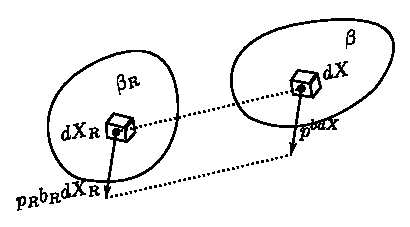
\includegraphics{vol71-figures/fig1.2-4.eps}
\medskip
\caption{}\label{fig1.2.4}
\end{figure}

By the principle of conservation of mass, it is known that 
$$
\rho_R(X_R) dX_R = \rho(X) dX.
$$

By defining
\begin{equation*}
b_R(X_R) = b(X), \text{or} b_R = b o \phi \tag{1.2-15}\label{eq1.2-15}
\end{equation*}
it follows that
$$
\rho_R b_R dX_R = \rho b dX.
$$

Note that, \textit{a priori}, $b_R$ depends on $\phi$.

\begin{remark}\label{chap1-rem1.2.3}%Remark 1.2-3
Since it is known that $dX = \det (\nabla  \phi) dX_R$, it follows that
\begin{equation*}
  \rho(X) = \frac{\rho_R (X_R)}{\det \nabla
    \phi(X_R)}.\tag{1.2-16}\label{eq1.2-16} 
\end{equation*}
\end{remark}

Since\pageoriginale  the density at any point (in either
configuration) has to be 
finite and positive, this, if not any other, is a necessary reason for
a deformation to satisfy. $\det (\nabla  \phi) \neq 0$. 

Multiplying equation \eqref{eq1.2-7} by det $(\nabla  \phi)$ on both
sides, it follows that 
\begin{equation*}
DIV_R T_R + \rho_R b_R = 0 ~\text{in}~
\mathfrak{B}_R\tag{1.2-17}\label{eq1.2-17}
\end{equation*}

Thus the divergence form is preserved. Note however that $T_R$ is
\textit{not} symemetric. A \textit{symmetric} tensor to $T_R$ can be
defined. It is the \textit{second Piola-Kirchhoff stress
  tensor},\index{Piola-Kirchhoff stress tensors}\index{stress!PIOLA-KIRCHHOFF - tensors} $\sum_R$, given by  
\begin{equation*}
\sum_R = \det (\nabla  \phi) (\nabla  \phi)^{-1}
T(\nabla  \phi)^{-T}\tag{1.2-18} \label{eq1.2-18}
\end{equation*}

It is related to $T_R$ by 
\begin{equation*}
\sum_R = (\nabla  \phi)^{-1} T_R.\tag{1.2-19}\label{eq1.2-19}
\end{equation*}

\begin{remark}\label{chap1-rem1.2.4}% Remark 1.2-4
It is understandable that $T_R$ is not symmetric as it belongs partly
to the reference configuration and partly to the deformed
configuration and symmetry does not make much sense in such a
situation. 
\end{remark}

Now we turn to the transformation of the surface forces. The
\textit{first Piola-Kirchhoff stress vector}\index{Piola-Kirchhoff stress vector}\index{stress!PIOLA-KIRCHHOFF - vector} is defined so that 
\begin{equation*}
t_R(X_R, n_R) = T_R(X_R) n_R.\tag{1.2-20}\label{eq1.2-20}
\end{equation*}
\begin{figure}[H]
\centering
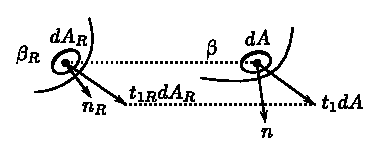
\includegraphics{vol71-figures/fig1.2-5.eps}
\medskip
\caption{}\label{fig1.2.5}
\end{figure}

Recall\pageoriginale  that $T_R (X_R) n_R dA_R = T(X) ndA$ and so 
$$
t_R(X_R,n_R) dA_R = t(X,n)dA.
$$

If $\partial \mathfrak{B}_{1R}$ is the portion of
$\partial\mathfrak{B}_R$ mapped by $\phi$ onto
$\partial\mathfrak{B}_1$, define $t_{1R} : \partial\mathfrak{B}_{1R}
\rightarrow \mathbb{R}^3$ by $t_{1R} dA_R = t_1 dA$. Again, \textit{a
  priori}, $t_{1\mathbb{R}}$ depends on $\phi$. Explicitly, by Theorem
\ref{chap1-thm1.1.1}, 
\begin{equation*}
  t_{1R(X_R)} = \det  (\nabla  \phi (X_R)) | (\nabla  \phi
  (X_R))^{-T} n_R | t_1 (\phi (X_R)).\tag{1.2-21}\label{eq1.2-21} 
\end{equation*}

The following result is easy to establish.

\begin{theorem}\label{chap1-thm1.2.3}%Theorem 1.2-3
The equilibrium equations\index{equilibrium equations} in the reference configuration are given by  
\begin{align*}
 DIV_R T_R + \rho_R b_R & = o  ~\text{in}~
 \mathfrak{B}_R\tag{1.2-22}\label{eq1.2-22}\\ 
  (\nabla  \phi ) T^T_R &= T_R (\nabla  \phi)^{T}  ~\text{in}
  \mathfrak{B}_R\tag{1.2-23}\label{eq1.2-23}\\ 
  T_R n_R & = t_{\mathbb{R}}  on  \partial
  \mathfrak{B}_{\mathbb{R}}.\tag{1.2-24}\label{eq1.2-24} 
\end{align*}

Equivalently, in terms of $\sum_R$
\begin{align*}
  DIV_R (\nabla  \phi\sum_R) + \rho_R b_R & = 0  ~\text{in}~
  \mathfrak{B}_R\tag{1.2-25}\label{eq1.2-25}\\
  \sum_R & = \sum_R^T ~\text{in}~ \mathfrak{B}_R\tag{1.2-26}\label{eq1.2-26}\\
  \nabla  \phi \sum_R n_R & = t_{1\mathbb{R}}  ~\text{on}~  \partial
  \mathfrak{B}_{1\mathbb{R}}.\hspace{1cm}\tag{1.2-27}\label{eq1.2-27} 
\end{align*}

Again, this is equivalent to the variational equations 
\begin{equation*}
  \int\limits_{\mathfrak{B}_R} T_R : \nabla  \theta  dX_R =
  \int\limits_{\mathfrak{B}_R} \rho_R b_R.\theta dX_R +
  \int\limits_{\partial \mathfrak{B}_{1R}} t_{1R}.\theta dA_R
  \tag{1.2-28} \label{eq1.2-28}
\end{equation*}
for all $\theta : \mathfrak{B}_R \rightarrow \mathbb{R}^3$ vanishing
on $\partial \mathfrak{B}_{oR} = \partial \mathfrak{B}_R \backslash
\partial \mathfrak{B}_{1\mathbb{R}}$. 
\end{theorem}

\begin{remark}\label{chap1-rem1.2.5}%Remark 1.2-5
Equations\pageoriginale \eqref{eq1.2-28} go under the name of the
principle of virtual work\index{principle of virtual work} in the reference configuration. 
\end{remark}

To conclude this section, some classes of applied forces are
considered. Recall that while $\rho_R$ is completely known, $b_R$ and
$t_{1\mathbb{R}}$ depend in general on $\phi$ which is unknown. 

A body force\index{body force}\index{force: applied surface!body} (resp. applied surfaces force) is a
\textit{dead load}\index{dead load} if 
$b_R$ (resp. $t_{1R}$) is a function of $X_R$ only, independent of
$\phi$. 

An example of a body force which is a dead load is gravity which is
constant; $b = (o,o,-g)$. A trivial example of an applied surface
force which is a dead load is $t_1 = 0!$ The pressure\index{pressure} is an example of
an applied surface force which is \textit{not} a dead load: 
\begin{equation*}
t_1 = - pn\tag{1.2-29}\label{eq1.2-29}
\end{equation*}
where $p > o $ indicates an inward directed force (pressure) and $p <
0 $ indicates one which is directed outward (traction). Now 
$$
t_{1R} = - p \det (\nabla\phi) (\nabla\phi)^{-T} n_R
~\text{on}~ \partial\mathfrak{B}_R 
$$
which clearly depends on $\phi !$

A body force is said to be \textit{conservative}\index{conservative body force} if there exists a
function $\beta : \mathbb{R}^3 \times \mathfrak{B}_R \to \beta(\phi,
X_R) \epsilon \mathbb{R}$, such that 
\begin{equation*}
b_R(X_R) = \nabla_{\phi}\beta(\phi(X_R),X_R), \tag{1.2-30}\label{eq1.2-30}
\end{equation*}
for all $X_R \epsilon \mathfrak{B}_R$ and all deformations
$\phi$. If which is the case then  
\begin{equation*}
  \int\limits_{\mathfrak{B}_R} \rho_R b_R.\theta dX_R = B(\phi)
  (\theta)\tag{1.2-31} \label{eq1.2-31}
\end{equation*}
where
\begin{equation*}
  B(\psi) = \int\limits_{\mathfrak{B}_R} \rho_R (X_R)
  \beta(\psi(X_R),X_R) dX_R.\tag{1.2-32} \label{eq1.2-32}
\end{equation*}\pageoriginale
\textit{A body force which is a deal load is conservative},
$\beta(\Phi,X_R) = b_R (X_R)$. $\Phi$. 

An applied surface\index{force: applied surface} force\index{applied surface force} is
\textit{conservative} if there exists a\index{conservative applied
  surface force}
function $\tauup_1 : \mathbb{R}^3 \times \partial \mathfrak{B}_{1R}
\rightarrow \tauup_1 (\phi,X_R) \epsilon \mathcal{R}$ such that 
\begin{equation*}
t_{1R}(X_R) = \nabla_{\Phi} \tauup_1
(\phi(X_R),X_R).\tag{1.2-33}\label{eq1.2-33} 
\end{equation*}

Then again
\begin{equation*}
\int\limits_{\partial\mathfrak{B}_{1R}} t_{1R}.\theta dA_R =
T'_1(\phi)(\theta)\tag{1.2-34} \label{eq1.2-34}
\end{equation*}
where
\begin{equation*}
T_1(\psi) = \int\limits_{\partial\mathfrak{B}_{1R}}
\tauup_1(\psi(X_R),X_R) dA_R.\tag{1.2-35} \label{eq1.2-35}
\end{equation*}

\textit{An applied surface force which is a deal load is
  conservative};\hfill\break $\tauup_1 (\phi,X_R) = t_{1\mathbb{R}}(X_R).\Phi$. A
pressure load is conservative (Exercise 1.2-3). 

\medskip
\begin{center}
{\large\bf Exercises}
\end{center}

\begin{description}
\item[1.2-1]. (Da Silva's Theorem).\index{Da Silva's Theorem} Given
  any system of applied 
  forces (with $\partial\mathfrak{B}_1 = \partial\mathfrak{B}$) show
  that there exists $Q \epsilon \mathbb{O}^3$ such that  
  \begin{align*}
    & \int\limits_{\mathfrak{B}} \rho(X) OX \Lambda Q b(X)dX +
    \int\limits_{\partial \mathfrak{B}} OX \Lambda Q t(X) dA = o\\ 
    & \int\limits_{\mathfrak{B}}  \rho(X) Q^T(OX) \Lambda b(X)dX +
    \int\limits_{\partial \mathfrak{B}} Q^T(OX) \Lambda t(X)dA = o. 
  \end{align*}

How many solutions exist?

\item[1.2-2.] Show that the fundamental axiom of static equilibrium\index{axiom of static equilibrium}
  is equivalent to  
  $$
  \int\limits_{\vartheta}\rho(X) b(X).v(X)dX +
  \int\limits_{\partial\vartheta} t(X,n).v(X) dX = 0 
  $$\pageoriginale
for every volume $\vartheta \subset \mathfrak{B}$ and for every
\textit{infinitesimal rigid displacement}\index{infinitesimal rigid
  displacement}  $v$, i.e., 
  $$
   v(x) = a + b \Lambda O x,a,b \epsilon \mathbb{R}^3.
  $$

This is sometimes also called the principle of virtual work.\index{principle of virtual work} $1.2-3$. 

\item[1.2-3]Show that a pressure\index{pressure} load is conservative.
\end{description}

\section{Constitutive Equations}\label{chap1-sec1.3}%SECTION 1.3
\setcounter{figure}{0}

Given a body acted on by a system of forces, one's main objective is
to compute the deformation $\phi$ which has $3$ component
functions. As a natural \textit{intermediary}, the stress tensor $T$
has come in which has 6 components (taking into account its
symmetry). But so far, the boundary value problem obtained via the
equilibrium equations has yielded only $3$ equations
(cf. \eqref{eq1.2-7}). Thus 6 more equations must be found. 

From the physical point of view, observe that in obtaining the
equilibrium equations, no property of the material under consideration
has been used. Since different materials react differently to the same
forces, obviously these equations alone cannot describe the response of
the material. 

Thus one is led to finding more equations to complete the system. A
material is said to be \textit{elastic}\index{elastic material}\index{material!elastic} if there exists a mapping  
$$
\hat{T} : F \epsilon \mathbb{M}^3_+ \to \hat{T}(F) \epsilon \mathbb{S}^3
$$
such\pageoriginale that for any deformed configuration and any point $X=\phi(X_R)$, 
\begin{equation*}
T(X)= \hat{T}(\nabla \Phi(X_R) ). \tag{1.3-1}\label{eq1.3-1}
\end{equation*}

The map $\hat{T}$ is called the \textit{response function}\index{response function} and
\eqref{eq1.3-1} is called a \textit{constitutive
  equation.}\index{constitutive equation}  

\begin{remark}\label{chap1-rem1.3.1} %Remark 1.3-1
The map $\hat{T}$ above does not depends explicitly on $X_R$. Such
that a material is called \textit{homogeneous.}\index{homogeneous
  material}\index{material!homogeneous} If it were that   
$$
T(X)= \hat{T}(X_R, \nabla \Phi (X_R))
$$
the material would be called a
\textit{non-homogeneous}\index{material!non-homogeneous}\index{non-homogeneous
material} elastic material. 
\end{remark}

If $T_R$ is the Piola transform of $T$ then it follows that 
\begin{equation*}
  T_R= \det (\nabla \phi)\hat{T}(\nabla \phi
  )(\nabla \phi)^{-1} \overset{\de}{=} \hat{T}_R(\nabla
  \phi) \tag{1.3-2} \label{eq1.3-2}
\end{equation*}
which gives a reponse fucntion $\hat{T}_R : \mathbb{M}^3_+ \to
\mathbb{M}^3$ for $T_R$. Similarly it is possible to write one for
$\Sigma_R$ in terms of a response function $\hat{\Sigma}_R:
\mathbb{M}^3_+ \to \mathbb{S}^3$.  

\begin{theorem}[Polar Factorisation]\label{chap1-thm1.3.1}%thm 1.3-1
Let\index{polar factorisation of a matrix} $F$ be an invertible matrix. Then
there exist an orthogonal matrix $R$ and symmetric, positive definite
matrices $U$ and $V$ such that  
\begin{equation*}
  F=RU=VR. \tag{1.3-3}\label{eq1.3-3}
\end{equation*}

Such a factorization is unique. 
\end{theorem}

\begin{proof}
Cf. Exircise 1.3-1. 
\end{proof}

\begin{dashremark}%Remark 1.3-1
If $F \in \mathbb{M}^3_+$ then $R \in , \mathbb{O}^3_+$. If $G \in
\mathbb{S}^3_>$ there exists a unique matrix $H \in \mathbb{S}^3_>$
such that $H^2=G$. It is usual to write $H =G^{1/2}$. It can be seen
that $U=(F^TF)^{1/2}$ and $V= (FF^T)^{1/2}$, in\pageoriginale the above
theorem. Since $V= R U R^T, U$ and $V$ are similar. Then so are $B
=FF^T$ and $C=F^TF$.  
\end{dashremark}

The constitutive equation \eqref{eq1.3-1} can be written componentwise as 
$$
T_{ll}(X)= \hat{T}_{ll} \left( \frac{\partial \phi_1}{\partial
  X_{R_1}}(X_R), \ldots , \frac{\partial \phi_3}{\partial
  X_{R_3}}(X_R)\right) 
$$
and so on. So knowing $\hat{T}$ is the same as knowing the functions
$\hat{T}_{ij}$. However, the functions $\hat{T}_{ij}$ cannot be chosen
arbitrarily. They must somehow reflect an \textit{intrinsic} property
of the material in equation, irrespective of the coordinate system
chosen. This is the idea embodying the  

\medskip
\noindent
\textit{AXIOM OF MATERIAL FRAME INDIFFERENCE}.\index{axiom of material
  frame indifference}\index{material frame indifference} \textit{The Cauchy
  stress vector\index{Cauchy stress vector}\index{stress!CAUCHY - vector} $t(X, n)= T(X)n$ should be
  independent of the 
  particular basis in which the constitutive equation is expressed.} 

\begin{theorem}\label{chap1-thm1.3.2} %Theorem 1.3-2
The following are equivalent. 
\begin{enumerate}[\rm(i)]
\item A response function $\hat{T}: \mathbb{M}^3_+ \to \mathbb{S}^3$
  satisfies the axiom of material frame indifference.  
\item For every $Q \in \mathbb{O}^3_+$ and for every $F \in \mathbb{M}^3_+$, 
  \begin{equation*}
    \hat{T}(QF)= Q \hat{T}(F)Q^T. \tag{1.3-4}\label{eq1.3.4}
  \end{equation*}
\item For every $F \in \mathbb{M}^3_+$ if $F=RU$ is its polar
  factorisation then  
  \begin{equation*}
    \hat{T}(F)= R \hat{T}(U)R^T \tag{1.3-5}\label{eq1.3.5}
  \end{equation*}
\item There exists a map $\tilde{\Sigma}_R: \mathbb{S}^3_> \to
  \mathbb{S}^3$ such that  
  \begin{equation*}
    \tilde{\Sigma}_R (F)= \tilde{\Sigma}_R(F^T F) \tag{1.3-6}\label{eq1.3-6}
  \end{equation*}\pageoriginale
  for every $F \in \mathbb{M}^3_+$. 
\end{enumerate}
\end{theorem}

\begin{proof}
(i) $\Leftrightarrow$ (ii) Instead of rotating the coordinate axes the
  same effect can be achived by rotating the deformed configuration.
\end{proof}

\begin{figure}[H]
\centering
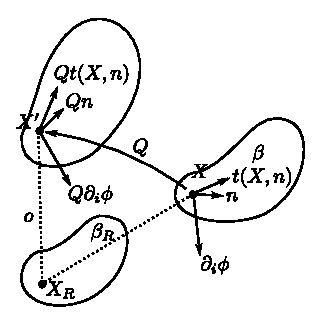
\includegraphics{vol71-figures/fig1.3-1.eps}
\medskip
\caption{}\label{fig.1.3.1}
\end{figure}

Rotating $\mathcal{B}$ by a map $Q \in \mathbb{O}^3_+$, let $X$ map
into $X'$. The normal $n$ at any goes to $Qn$ and $t(X, n)$ goes to
$Qt(X, n)$. Thus  
\begin{align*}
t(X', Qn)& = T' (X')Qn\\
t(X', Qn)& = Q t(X, n)= QT(X)n. \\
\end{align*}\pageoriginale
Since $n$ is arbitrary, it follows that 
\begin{equation*}
T'(X')=QT(x)Q^T \tag{1.3-7}\label{eq1.3-7}
\end{equation*}

Thus 
$$
\hat{T}(Q \nabla \phi(X_R))= Q \hat{T}(\nabla \phi(X_R)) Q^T
$$
for any $Q \in \mathbb{O}^3_+$ and any $F =\nabla \phi \in
\mathbb{M}^3_+$. This shown that (i) $\Rightarrow$ (ii) Simply
retracting the argument proves the converse.  

(ii) $\Leftrightarrow$ (iii). If $F= RU$, then by (ii),
since $R \in \mathbb{O}^3_+$
$$
\hat{T}(RU)= R \hat{T}(U)R^T
$$
which is (iii). Conversely, assuming (iii), if $F=RU$ then the
polar factorization $QF$ is $(QR)U$ for $Q \in \mathbb{O}^3_+$, as the
factorization is unique. Thus 
$$
\hat{T}(QF)= QR \hat{T}(U) R^T Q^T = Q\hat{T}(F)Q^T. 
$$ 
(ii) $\Leftrightarrow$ (vi). Since $F=RU$ implies $U=(F^TF)^{1/2}$, 
\begin{align*}
  \hat{T}(F)&= R \hat{T}(U)R^T\\
  &= FU^{-1} \hat{T}(U)U^{-1} F^T\\
  &= F \tilde{S} (F^T F) F^T\\
\end{align*}
where $\tilde{S}: \mathbb{S}^3_> \to \mathbb{S}^3$. Conversely, if
$\hat{T}(F)$ is of the above form, then if $F=RU$,  
$$
\hat{T}(U)= U \tilde{S}(U^2)U
$$\pageoriginale
and 
 \begin{align*}
   \hat{T}(F)&= F \tilde{S}(F^T F) F^T\\
   &= F \tilde{S}(U^2) F^T\\
   &= F U^{-1}\hat{T}(U) U^{-1} F^T\\
   &= R \hat{T}(U) R^T. 
 \end{align*} 
 Now
 \begin{align*}
\Sigma_R (F) &= \det (F) F^{-1} \hat{T}(F) F^{-T}\\
&= (\det (F^TF))^{1/2} \tilde{S}(F^TF)= \tilde{\Sigma}_R (F^T F). 
 \end{align*} 

\begin{remark}\label{chap1-rem1.3.2} %Remark 1.3-2
If one of the response functions, say $\Gamma$, can be written of
either variables $F, F^T F=C, FF^T =B$ or $E$ ( where $C=I+2E $), the
following notation will be employed when the different dependences are
expressed: 
$$
\Gamma = \hat{\Gamma}(F)= \tilde{\Gamma}(F^TF)= \bar{\Gamma}(FF^T)= \Gamma^*(E)
$$
\end{remark}

In the above theorem it has been proved that it is enough to know the
action of $\hat{T}$ on a relatively small class of matrices like
$\mathbb{S}^3_>$.

A material or response function is said to be
\textit{isotropic}\index{isotropic material}\index{isotropic response
  function}\index{material!isotropic} if 
the Cauchy strees tensor (or vector) computed at a given point in the
deformed configuration is the same if the same if the reference
configuration is rotated by any rigid defomation.

While the axiom of material frame indifference is an \textit{axiom} to
verified by any response fucntion, isotropy is a \textit{property} of
a particular material. There can be materials which are non-isotropic;
for instance, a body up of layers of different materials.

\begin{theorem}\label{chap1-thm1.3.3} %Theorem 1.3-3
	The\pageoriginale following are equivalent. 
\begin{enumerate}[\rm(i)]
\item A response function $\hat{T}: \mathbb{M}^3_+ \to \mathbb{S}^3$
  is isotropic.  
\item For every $F \in \mathbb{M}^3_+$ and for every $Q \in \mathbb{O}^3_+$, 
\begin{equation*}
\hat{T}(F)= \hat{T}(FQ). \tag{1.3-8}\label{eq1.3-8}
\end{equation*}
\item There exists a map $\bar{T}: \mathbb{S}^3_> \to \mathbb{S}^3$
  such that for every $F \in \mathbb{M}^3_+$, 
 \begin{equation*}
\hat{T}(F)= \bar{T}(FF^T). \tag{1.3-9}\label{eq1.3-9}
 \end{equation*}
\end{enumerate}
\end{theorem}

\begin{proof}
(i) $\Leftrightarrow$ (ii). Let $Q \in
\mathbb{O}^3_+$. Rotate the 
  reference configuration about a point $\bar{X}_R$ so that if $X_R
  \in \mathfrak{B}_R$ then
\begin{equation*}
  \theta(X_R)= \bar{X}_R + Q^T(\bar{X}_R X_R). \tag{$\Box$}
\end{equation*}

Then 
$$
\phi^* = \phi o \theta^{-1}. 
$$

\begin{figure}[H]
\centering
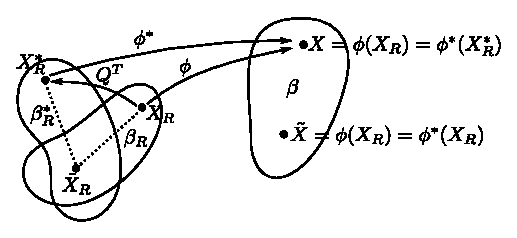
\includegraphics{vol71-figures/fig1.3-2.eps}
\medskip
\caption{}\label{fig1.3.2}
\end{figure}

The response function is isotropic if and only if 
$$
\displaylines{\hfill
\hat{T}(\bar{X})= \hat{T}( \nabla \phi(\tilde{X}_R)) = \hat{T}(
\nabla \phi^* ( \tilde{X}_R)) \hfill\cr
\text{i.e.,} \hfill 
\tilde{T}(\nabla \phi(\tilde{X}_R)) = \hat{T}(\nabla
\phi( \bar{X}_R)Q).  \hfill}
$$\pageoriginale
(ii) $\Leftrightarrow$ (iii). Let $FF^T = GG^T, F, G \in
\mathbb{M}^3_+$. Then $G^{-1}F \in \mathbb{O}^3_+$. Hence by (ii) 
$$
\hat{T}(G)= \hat{T}(G(G^{-1}F)) = \hat{T}(F). 
$$

So it is clear that $\hat{T}(F)$ depends only on $FF^T$. Conversely if
$\hat{T}(F)= \bar{T}(FF^T)$ then for $Q \in \mathbb{O}^3_+$,  
$$
\hat{T}(FQ)= \bar{T}(FQQ^TF^T)= \bar{T}(FF^T)= \hat{T}(F). 
$$
\end{proof}


\begin{remark}\label{chap1-rem1.3.3}
By the axiom of material frame indifference, the constitutive equation
could be expreesed in terms of a function of $C=F^TF$ and this
involved rotating the \textit{deformed}configuration
$\mathfrak{B}$. By isotropy, the same could be expressed in terms of a
function of $B=FF^T$ and this involved rotating the \textit{reference}
configuration $\mathfrak{B}_R$. Thus these two nations seem to be
`dual' ot each other. 
\end{remark}

\begin{remark}\label{chap1-rem1.3.4} %Remark1.3-4
For non-isotropic materials it can be shown that 
$$
\hat{T}(F)= \hat{T}(FQ)
$$
for all $F \in \mathbb{M}^3_+$ but $Q$ variying over a subgroup of
$\mathbb{O}^3_+$.
\end{remark}

\textit{In what follows, the material will allways be assumed to be
  isotropic}. 

Before proving a very powerful and elgent result on the structure of a
reponse function which is isotrophic and material frame-indifferent,
the following definition is needed.

Let $A \in \mathbb{M}^3$. Define $\imath_A$ to be the triple $(\imath_1(A),
\imath_2(A), \imath_3(A))$ where $\imath_1(A), \imath_2(A)$ and $\imath_3(A)$ \textit{are the
  principal invariants of}\index{principal invariants of a matrix} $A$, and  
\begin{align*}
  \det (A- \lambda I) & =- \lambda^3 +\imath_1(A) \lambda^2 -
  \imath_2(A) \lambda + 
  \imath_3(A). \tag{1.3-10}\label{eq1.3-10}
\end{align*}

If $A =(a_{ij})$ and $\lambda_1, \lambda_2, \lambda_3$ are its
eigenvalues, then  
\begin{align*}
  \imath_1(A) & = a_{ii}= tr(A)= \lambda_1 + \lambda_2 +
  \lambda_3. \tag{1.3-11}\label{eq1.3-11}\\ 
  \imath_2(A)& = \frac{1}{2}(a_{ii}a_{jj}- a_{jj}a_{ij}) =\frac{1}{2}((
  tr(A))^2- tr(A^2))\\ 
  & \qquad = \tr (\adj  A)= \lambda_1 \lambda^2 + \lambda_2
  \lambda_3 + \lambda_3 \lambda_1. \tag{1.3-12}\label{eq1.3-12} \\
  \imath_{3}(A) & = \det (A) = \frac{1}{6}((tr(A))^3- 3tr(A) tr(A^2) +
  2tr(A^3))= \lambda_1 \lambda_2 \lambda_3. \tag{1.3-13} \label{eq1.3-13}
\end{align*}\pageoriginale

 Further, if $A$ is invertible, 
 \begin{equation*}
   \imath_2(A)= (\det A) tr(A^{-1}). \tag{1.3-14}\label{eq1.3-14}
 \end{equation*} 
 
 The following theorem is one of the most important results in the
 theorey of elasticity.
  
 \begin{theorem}[Rivlin-Ericksen Theorem]\label{chap1-thm1.3.4}
   \index{Rivlin-Ericksen Theorem}
    A response function $\hat{T}:
   \mathbb{M}^3_+ \to \mathbb{S}^3$ is isotropic\index{isotropic
     response function} and material frame
   indifferent\index{material frame indifference} if, and only if, it is of the $\hat{T}(F)= \bar{T}(FF^T)$
   where the mapping $\bar{T}: \mathbb{S}^3_> \to \mathbb{S}^3$ is of the
   form 
   \begin{equation*}
     \bar{T}(B)= \beta_o(\imath_B) I + \beta_1(\imath_B) B+\beta_2(\imath_B)B^2 \tag{1.3-15}\label{eq1.3-15}
   \end{equation*}
   for all $B \in \mathbb{S}^3_>$. where $\beta_o , \beta_1, \beta_2$ are
   real valued functions.  
 \end{theorem} 

 \begin{proof}
   (i) Let $\hat{T}: \mathbb{M}^3_+ \to \mathbb{S}^3$ be material frame
   indifferent and isotropic. Then by isotropy $\hat{T}(F)=
   \bar{T}(FF^T)$ for some mapping $\bar{T}: \mathbb{S}^3_> \to
   \mathbb{S}^3$. Let $Q \in \mathbb{O}^3_+$ and $B \in
   \mathbb{S}^3_>$. On one hand , by isotrophy 
   $$
   \hat{T}(QB^{1/2})= \bar{T}(QB^{1/2}B^{1/2}Q^T) = \bar{T}(QBQ^T). 
   $$ 

   On the other hand, by the material frame indifference, 
   \begin{align*}
     \hat{T}(QB^{1/2}) &= Q \hat{T}(B^{1/2}) Q^T\\
     &=Q \bar{T}(B^{1/2} B^{1/2}) Q^T= Q \bar{T}(B) Q. 
   \end{align*} \pageoriginale
   
   Thus $\bar{T}$ satisfies , for all $Q \in \mathbb{O}^3_+$, and $B \in
   \mathbb{S}^3_>$ 
   \begin{equation*}
     \bar{T}(QBQ^T)= Q \bar{T}(B)Q^T. \tag{1.3-16}\label{eq1.3-16}
   \end{equation*} 
   
   Conversly, let $\bar{T}: \mathbb{S}^3_> \to \mathbb{S}^3$ satisfy
   \eqref{eq1.3-16} and let $\hat{T}(F)= \bar{T}(F^TF)$. Then clearly,
   $\hat{T}$ is isotrophic. If $Q \in \mathbb{O}^3_+$, then  
   \begin{align*}
     \hat{T}(QF)&= \bar{T}(QFF^TQ^T) = Q \bar{T}(FF^T) QT. \\
     &= Q \hat{T}(F) Q^T
   \end{align*} 
   and so $\hat{T}$ is material frame indefferent. 
   
   Thus it is now enough to check that a mapping $\bar{T}: \mathbb{S}^3_>
   \to \mathbb{S}^3$ satisfying \eqref{eq1.3-16} is of the form
   \eqref{eq1.3-15}. (The converse is immediate to varify).  

\medskip   
 (ii)~ Let $\bar{T}: \mathbb{S}^3_> \to \mathbb{S}^3$ varify
   \eqref{eq1.3-16}. It will now be shown that any matrix which
   diagonalizes $B \in \mathbb{S}^3_>$ also diagnalizes
   $\bar{T}(B)$, i.e., any  eigenvector of $B$ is an eigenvector of
   $\bar{T}(B)$.   
   
   Let $B \in \mathbb{S}^3_>$ and $Q \in \mathbb{O}^3_+$ (we can always
   assume that) such that  
   $$
   Q^T BQ = \text{diag}~ (\lambda_i)
   $$
   where $\lambda_1, \lambda_2, \lambda_3$ are the eigenvalue of $B$. Define
   $$
   Q_1 = \text{diag}~ (1, -1, -1), Q_2 = \text{diag}~  (-1, 1, -1),
   Q_3= \text{diag}~ (-1, -1, 1).  
   $$

   Then $Q_k \in \mathbb{O}^3_+, k= 1, 2, 3$. 
   
   Also,\pageoriginale 
   $$
   Q^T_k Q^T BQQ_k= \text{diag}~ \lambda_i = Q^T BQ. 
   $$

   So, 
   \begin{align*}
     Q^T_k Q^T \bar{T}(B) QQ_k &= \bar{T}(Q_k^T Q^T BQQ_k)\\
     &=\bar{T}(Q^T BQ)\\
     &= Q^T \bar{T}(B) Q. 
   \end{align*} 

   If $D=Q^T \bar{T}(B) Q$, then
   $$
   Q^T_k DQ_k = D, k= 1, 2, 3. 
   $$

   If the diagonal entries of $Q_k$ are $q^k_i(=1 ~\text{if}~ i=k, -1
   ~\text{if}~ i \neq k)$, then it follows that  
   $$
   D_{ij}= q^k_i D_{ij} q^k_j ~\text{for all}~ 1 \leq i, j, k \leq 3. 
   $$ 

   Thus if $i =k \neq j$, then 
   $$
   D_{kj}=- D_{kj} ~\text{or}~ D_{kj}=o. 
   $$
   Hence $D$ is diagonal and this proves the claim. 

\medskip   
 (iii)~ It will now be a shown that if $\bar{T}$ satisfies \eqref{eq1.3-16}
   then, for all $B \in \mathbb{S}^3_>$,  
   \begin{equation*}
     \bar{T}(B)= b_o(B) I + b_1(B)B+b_2(B)B^2, \tag{1.3-17}\label{eq1.3-17}
   \end{equation*} 
   $b_\alpha, \alpha = 0, 1, 2$ being real valued functions on
   $\mathbb{S}^3_>. $ 
 \end{proof}

\begin{case}\label{chap1-sec1.3-case1} %Case 1
 $B$\pageoriginale has 3 distanct eigenvalues $\lambda_1, \lambda_2,
  \lambda_3$ with corresponding orthonormal eigenvectors $p_1$,
  $p_2$, $p_3$. Then  
  \begin{align*}
    I & = p_1 p_1^T +p_1 p_2^T + p_3 p_3^T \tag{1.3-18}\label{eq1.3-18}\\
    B &=\lambda_1 p_1 p_1^T + \lambda_2 p_2p_2^T + \lambda_3 p_3 p_3^T
    \tag{1.3-19}\label{eq1.3-19} \\
    B^2 & = \lambda_1^2 p_1 p_1^T + \lambda_2^2 p_2p_2^T + \lambda_3^2 p_3
    p_3^T \tag{1.3-20} \label{eq1.3-20}
  \end{align*}
\end{case}

Since the $\lambda_i$ are distinct, the Vandermonde determinant
$$
\det
\begin{bmatrix}
1 & 1 & 1\\
\lambda_1 &\lambda_2 &\lambda_3\\
\lambda^2_1 &\lambda^2_2 &\lambda_3^2
 \end{bmatrix}
 $$ 
is non-zero and so in $\mathbb{S}^3$, the span of $p_i p_i^T, i= 1, 2,
3$ is equal to that of $I, B, B^2$. But $\bar{T}(B)$, by step (ii)
above, has the same eigenvectors as $B$. So  
 \begin{equation*}
   \bar{T}(B)= \mu_1 p_1p_1^T + \mu_2 p_2p_2^T + \mu_3p_3 p_3^T
   \tag{1.3-21}\label{eq1.3-21} 
 \end{equation*} 
 which implies that $\bar{T}(B) \in$ span $\{I, B, B^2 \}$. 

\begin{case}\label{chap1-sec1.3-case2} %CAse 2
  $\lambda_1 \neq \lambda_2 = \lambda_3$. Again one can write
   \eqref{eq1.3-18} and \eqref{eq1.3-19}. Then the span of $p_1 p_1^T$ and $p_2
   p_2^T +p_3p_3^T$ is that of $I$ and $B$. By step (ii), it can be
   seen that $\mu_2= \mu_3$, since any non-zero vector spanned by
   $p_2$ and $p_3$ is also an eigenvector for $\bar{T}(B)$. Thus in
   \eqref{eq1.3-21} 
   $$
   \bar{T}(B)= \mu_1 p_1 p_1^T + \mu_2 (p_2p_2^T + p_3 p_3^T)
   $$
   which shows $\bar{T}(B) \in$ span $(I, B)$. 
\end{case} 

 \begin{case}\label{chap1-sec1.3-case3} %Case 3
   $\lambda_1 = \lambda_2 = \lambda_3$.\pageoriginale In this case,
   one can similarly 
   see that $B, \bar{T}(B)$ are both scalar multiples of $I$.  
 \end{case} 
 
 (iv) Case. \ref{chap1-sec1.3-case1}. $\lambda_1, \lambda_2,
 \lambda_3$ are distinct 
 eigenvalues of $B \in \mathbb{S}^3_>$, .  
  
 Let $Q \in \mathbb{O}^3_+$. 
 \begin{align*}
   \bar{T}(QBQ^T)&= b_o (QBQ^T) I+b_1 (QBQ^T) QBQ^T +b_2 (QBQ^T) QB^2Q^T\\
   &= Q(b_o (QBQ^T)I + b_1(QBQ^T)B+b_2(QBQ^T)B^2)Q^T
 \end{align*} 
 But
 $$
 \bar{T}(QBQ^T)= Q\bar{T}(B) Q^T = Q(b_o(B)I +b_1(B)B+b_2(B)B^2)Q^T. 
 $$

 Thus $b_\alpha: \mathbb{S}^3_> \to \mathbb{R}, \alpha= 0, 1, 2$
 satisfy the functional identity  
 \begin{equation*}
   b_\alpha(QBQ^T)=b_\alpha(B) \tag{1.3-22}\label{eq1.3-22}
 \end{equation*} 
 for all $B \in \mathbb{S}^3_>$ and for all $Q \in
 \mathbb{O}^3_+$. Thus if $Q$ diagnalizes $B$, it is seen that such a
 function $b_\alpha$ must be a function of the eigenvalues of $B$
 only. Now choosing $Q_i \in \mathbb{O}^3_+, i = 1, 2, 3$ as
 $$
 Q_1=
 \begin{bmatrix}
   0 & 1 & 0 & \\
   1 & 0 & 0 \\
   0 & 0 & -1
 \end{bmatrix} , 
 Q_2=
 \begin{bmatrix}
   -1 & 0 & 0\\
   0& 0 &1\\
   0& 1& 0 
 \end{bmatrix} , 
 Q_3= 
 \begin{bmatrix}
   0& 0& 1\\
   0 & -1 &0\\
   1 &0 &0
 \end{bmatrix} 
 $$
 it is seen from \eqref{eq1.3-22} that $b_\alpha$ is a symmetric function of
 $\lambda_1, \lambda_2, \lambda_3$. i.e,. $b_\alpha(B)= \beta_\alpha(t_{B})$.
 
This proves the theorem completely.  

 \begin{theorem}\label{chap1-thm1.3.5} %Theorem 1.-5.
   (a) Given $\mathfrak{B}_R$ and an isotropic material frame
   indifferent\index{material frame indifference} material, then in any deformed configuration
   $\mathfrak{B}= \phi(\mathfrak{B}_R)$, the Cauchy stress
   tensor\index{Cauchy stress tensor}\index{stress!CAUCHY - tensor} is
   given by  
\begin{equation*}
T(X) = \hat{T}(\nabla \phi(X_R)) = \bar{T}(\nabla \phi
(X_R)\nabla \phi (X_R)^T), \tag{1.3-23} \label{eq1.3-23}
\end{equation*}\pageoriginale

$\bar{T} : \mathbb{S}^3_> \rightarrow \mathbb{S}^3$
\textit{satisfying} \eqref{eq1.3-15}.  

(b)~ The second Piola-Kirchhoff stress tensor\index{Piola-Kirchhoff stress tensors}\index{stress!PIOLA-KIRCHHOFF - tensors} is given by 
\begin{equation*}
  \Sigma_R (X_R) = \hat{\Sigma_R}(\nabla \phi (X_R)) =
  \tilde{\Sigma_R}(\nabla\phi(X_R)^T \nabla \phi
  (X_R))\tag{1.3-24} \label{eq1.3-24}
\end{equation*}
\textit{where} $\tilde{\Sigma_R} : \mathbb{S}^3_> \to \mathbb{S}^3$
\textit{satisfies, for all} $C \in  \mathbb{S}^3_>$,  
\begin{equation*}
  \tilde{\Sigma_R}(C) = \gamma_o (\imath_c) I + \gamma_1 (\imath_c) C + \gamma_2
  (\imath_c) C^2. \tag{1.3-25} \label{eq1.3-25}
\end{equation*}
\end{theorem} 

\begin{proof}
  Observe that
  \begin{align*}
    \hat{\Sigma_R}(F) & = \det (F) F^{-1} \hat{T}(F) F^{-T}\\
    & = (\det (F^T F))^{1/2} F^{-1} \bar{T}(FF^T) F^{-T}\\
    & = (\det C)^{1/2} F^{-1}[\beta_O (\imath_B) I + \beta_1 (wr_B)B + B_2
      (\imath_B)B^2]F^{-T} 
  \end{align*}
  where $C = F^T F, B = FF^T$. But these are similar. So $\imath_B = \imath_c$. 

  Further 
  \begin{align*}
    & F^{-1} F^{-T} = C^{-1}\\
    & F^{-1}BF^{-T} = I\\
    & F^{-1} B^2F^{-T} = C. 
  \end{align*}
  
  By the Cayley-Hamilton theorem, 
  $$
  \displaylines{\hfill 
    -C^3 + \imath_1(C) C^2 - \imath_2(C) C + \imath_3(C) I = 0\hfill \cr
    \text{or}\hfill  
    C^{-1} = \frac{1}{\imath_3(C)} (C^2 - \imath_1(C) C + \imath_2(C)I)\hfill}
  $$
  where\pageoriginale $\imath_3(C) = \det C \neq 0$. Thus it is clear from these
  considerations that $\Sigma_R$ can be expressed in terms of $C$ as in
  \eqref{eq1.3-24} - \eqref{eq1.3-25}.  
\end{proof}

It was seen in Section \ref{chap1-sec1.1} that the Green-St
Venant\index{Green-St Venant strain tensor}\index{strain!Green-St Venant-tensor} strain tensor
$E$, given by $C = I + 2E$, `measures' the actual deformation. If
$\tilde{\Sigma_R}$ is sufficiently smooth it is possible to express it
in terms of $E$. More precisely, the following result is true.  

\begin{theorem}\label{chap1-thm1.3.6}%Theorem 1.3-6
  Let $\mathfrak{B}_R$ be the reference configuration of an isotropic,
  material frame indifferent elastic material. Assume that the functions
  $\gamma_{\alpha}, a = 0, 1, 2$ of \eqref{eq1.3-25} are differentiable at
  $\imath_I = (3, 3, 1)$. Then 
  \begin{equation*}
    \Sigma_R = \tilde{\Sigma_R}(I + 2E) = - pI + (\lambda(trE)I + 2\mu E)
    + O(E), \tag{1.3-26} \label{eq1.3-26}
  \end{equation*}
  where $p, \lambda$ and $\mu$ are constants. 
\end{theorem}

\begin{proof} %proof
Using the relations
\begin{align*}
\tr(C) & = 3 + 2\tr(E)\\
\tr(C^2) & = 3 + 4\tr(E) + o(E)\\
\tr(C^3) & = 3 + 6\tr(E) + o(E)
\end{align*}
and the relations \eqref{eq1.3-11} - \eqref{eq1.3-13}, it follows that 
\begin{align*}
\imath_1(C) & = 3 + 2\tr(E)\\
\imath_2(C) & = 3 + 4\tr(E) + o(E)\\
\imath_3(C) & = 1 + 2\tr(E) + o(E)
\end{align*}
so that
$$
\gamma(\imath_C) = \gamma(\imath_I) + (2
\frac{\partial\gamma}{\partial \imath_I} 
(\imath_I) + 4 \frac{\partial \gamma}{\partial \imath_2} (\imath_I)+ 2
\frac{\partial 
  \gamma}{\partial \imath_3} (\imath_I)) \tr(E) + O(E) 
$$
where\pageoriginale $\gamma = (\gamma_O, \gamma_1, \gamma_2)$. This yields
\eqref{eq1.3-26}. In particular 
\begin{align*}
  p & = - (\gamma_1 (\imath_I) + \gamma_1 (\imath_1) + \gamma_2
  (\imath_1)). \tag{1.3-27}\label{eq1.3-27}\\ 
  \lambda & = \sum_{\alpha = 0}^2  \left(2\frac{\partial
  \gamma_\alpha}{\partial \imath_1} (\imath_1) + 4 \frac{\partial
  \gamma_\alpha}{\partial \imath_2} (\imath_I) + 2 \frac{\partial
  \gamma_\alpha}{\partial \imath_3}
  (\imath_I)\right). \tag{1.3-28}\label{eq1.3-28}\\
  \mu &= \gamma_1 (\imath_1) + 2\gamma_2
  (\imath_1).\tag{1.3-29}\label{eq1.3-29} 
\end{align*}
\end{proof}

A reference configuration is a \textit{natural state}\index{natural state} if `there is no 
stress in it', i.e., $p = 0$. In this case 
\begin{equation*}
\Sigma_R = \Sigma^*_R(E) = \lambda \tr(E)I + 2 \mu E +
o(E)\tag{1.3-30}\label{eq1.3-30} 
\end{equation*}
and $\lambda$ and $\mu$ are called \textit{Lam\'e's
  constants}.\index{LAM\'E's constants} It is
possible to obtain \textit{a priori} some information on the nature of
the Lam\'e's constants.

Let $\mathfrak{B}_R$ be a natural state and have a `simple form'. Let
$\phi^{\in} : \mathfrak{B}_R \to \mathbb{R}^3$ be of the form 
\begin{equation*}
\phi^{\in}(X_R) = X_R + \in u(X_R) + o(\in ; X_R),
\tag{1.3-31}\label{eq1.3-31} 
\end{equation*}
where $\in > o$ is a small parameter, and where $\nabla u (X_R)
= G$, a \textit{constant} matrix. Such a deformation is a special case
of the so-called \textit{homogeneous
  deformations}\index{deformation}\index{homogeneous deformation}
where 
$\nabla \phi$ is a constant vector. Then 
\begin{align*}
T^{\in}(X) & = \hat{T}(I + \in G + o(\in ; X))\\
& = \hat{T}(I + \in G) + 0(\in ; X), X = \phi(X_R) . 
\end{align*}

Thus $DIV T^{\in}(X) = o(\in ; X)$ i. e. to within first order in
$\in$, \textit{there can be no body force}: such deformations can only
be produced by applied surface forces. Now it can be seen that  
\begin{equation*}
T^{\in}(X) = \in(\lambda(\tr G)I + \mu(G^T + G)) + o(\in
;X)\tag{1.3-32}\label{eq1.3-32} 
\end{equation*}\pageoriginale
using the fact that $\mathfrak{B}_R$ is a natural state. For
particular $\phi^\in$ considered the corresponding $T^\in$ is of some
simple form. This can be substituted in \eqref{eq1.3-32} and it is thus
possible to obtain inequalities for $\lambda$ and $\mu$.

\begin{experiment}\label{chap1-experiment1}% Experiment 1	
  Let $\mathcal{B}_R$ be a rectangular block. Choose 
  \begin{equation*}
    u^\in (X_R) \overset{\de}{=} \in u (X_R) = \in 
    \begin{bmatrix}
      X_{R_2}\\
      0 \\
      0 \\
    \end{bmatrix}. 
    \tag{1.3-33}
  \end{equation*}
\end{experiment}

Thus the body deforms as shown in figure~\ref{fig1.3.3}. 

\begin{figure}[H]
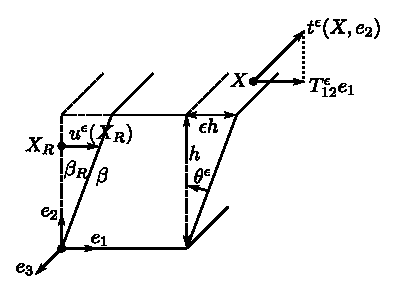
\includegraphics{vol71-figures/fig1.3-3.eps}
\medskip
\caption{}\label{fig1.3.3}
\end{figure}

Then it is logical to assume $T^{\in}_{12} = \in T_{12} + o(\in)$
where $T_{12} > o$. This follows from the interpretation of the
components of the stress tensor (cf. Remark
\ref{chap1-rem1.2.2}). Comparing 
this form with \eqref{eq1.3-32} if follows that  
\begin{equation*}
\mu > 0. \tag{1.3-34}\label{eq1.3-34}
\end{equation*}\pageoriginale

\begin{experiment}\label{chap1-experiment2}%Experiment 2	
Let $\mathfrak{B}_R$ be a sphere which is contracted by means of a
normal pressure.\index{pressure} Thus 
  \begin{equation*}
    u^\in (X_R) = \in
    \begin{bmatrix}
      -X_{R1}\\
      -X_{R2}\\
      -X_{R3}\\
    \end{bmatrix}
    + o(\in ; X_R). \tag{1.3-35}\label{eq1.3-35}
  \end{equation*}
\end{experiment}

Thus
\begin{equation*}
  T^\in(X) = - p \in I + o (\in ; X), p > 0. \tag{1.3-36}\label{eq1.3-36}
\end{equation*}

\begin{figure}[H]
\centering
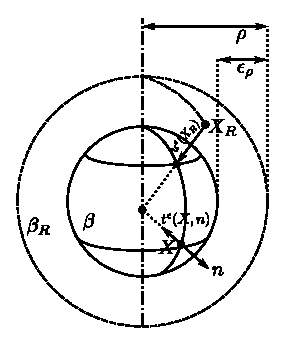
\includegraphics{vol71-figures/fig1.3-4.eps}
\medskip
\caption{}\label{fig1.3.4}
\end{figure}

It\pageoriginale can then be shown that 
\begin{equation*}
- p \in I = - \in (3 \lambda + 2\mu) I + 0(\in)\tag{1.3-37}\label{eq1.3-37}
\end{equation*}
from which it follows that
\begin{equation*}
3\lambda + 2\mu > 0. \tag{1.3-38}\label{eq1.3-38}
\end{equation*}

\begin{remark}\label{chap1-rem1.3.5}%Remark 1.3-5
  This precludes {\em{incompressible materials!}}\index{incompressible
    material}\index{material!incompressible} An example of an 
  incompressible material is rubber.
\end{remark}

\begin{experiment}\label{chap1-experiment3}% Experiment 3
  Let $\mathfrak{B}_R$ be a cylinder which is stretched as in
  figure~\ref{fig1.3.5}. 
  
  \begin{figure}[H]
    \centering
      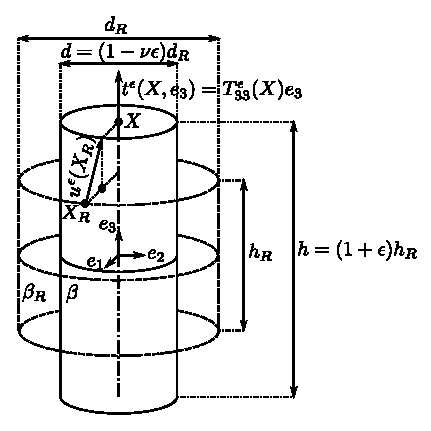
\includegraphics{vol71-figures/fig1.3-5.eps}
    \medskip
    \caption{}\label{fig1.3.5}
  \end{figure}
\end{experiment}

Now\pageoriginale
\begin{equation*}
  u^\in (X_R) = \in
  \begin{bmatrix}
    -\nu X_{R1}\\
    -\nu X_{R2}\\
    X_{R3}\\
  \end{bmatrix}
  + 0 (\in ; X_R), \nu > 0 \tag{1.3-39}\label{eq1.3-39}
\end{equation*}
and 
\begin{equation*}
  T^\in (X) = \in
  \begin{bmatrix}
    0 & 0 & 0\\
    0 & 0 & 0\\
    0 & 0 & E\\
  \end{bmatrix}
  + 0 (\in ; X). \tag{1.3-40}\label{eq1.3-40}
\end{equation*}

It can now be shown that 
\begin{equation*}
  \nu = \frac{\lambda}{2(\lambda + \mu )}, E = \frac{\mu(3\lambda +
    2\mu)}{\lambda + \mu}\tag{1.3-41}\label{eq1.3-41} 
\end{equation*}

Since $\mu > 0$ and $3\lambda + 2 \mu > 0$, it follows that $\lambda +
\mu > 0$. Since $\nu > 0$ it follows that  
\begin{equation*}
  \lambda > 0. \tag{1.3-42}\label{eq1.3-42}
\end{equation*}

Thus $\lambda > o$ and $\mu > 0$. (This does not make sense for
incompressible materials). The number $\nu$ is known as
\textit{Poisson's ratio}\index{Poisson's ratio} and $E$ as
\textit{Young's modulus}.\index{YOUNG's modulus} The
Lame's constants can be expressed in terms of these quantities:  
\begin{equation*}
\lambda = \frac{E \nu}{(1+\nu ) (1-2\nu )}, \mu =
\frac{E}{2(1+\nu)}. \tag{1.3-43} \label{eq1.3-43}
\end{equation*}

Thus $\lambda > O$ and $\mu > O$ is equivalent to 
\begin{equation*}
0 < \nu < 1/2, E > 0. \tag{1.3-44}\label{eq1.3-44}
\end{equation*}
(For an incompressible material, $\nu = 1/2$). 

An\pageoriginale elastic material is said to be a \textit{St
  Venant-Kirchhoff material}\index{material!St Venant-Kirchhoff}\index{St Venant-Kirchhoff material} if  
\begin{equation*}
\Sigma_R^*(E) = \lambda (\tr E)I + 2\mu E. \tag{1.3-45}\label{eq1.3-45}
\end{equation*}

It is also expressible in terms of $C$:
\begin{equation*}
  \tilde{\Sigma_R}(C) = \left\{\frac{\lambda}{2}(\imath_1(C) -3) - \mu
  \right\}I  + \mu C. \tag{1.3-46} \label{eq1.3-46}
\end{equation*}

Then the Cauchy stress tensor can be written as 
\begin{equation*}
  T = \bar{T}(B) = (\imath_3(B))^{1/2}\left\{\frac{\lambda}{2} (\imath_1(B)-3)
  -\mu\right\} B+\mu(\imath_1(B))^{1/2} B^2. \tag{1.3-47}\label{eq1.3-47} 
\end{equation*}

Thus such a material is isotropic and material frame indifferent
(cf. Theorem \ref{chap1-thm1.3.4}).  

\begin{remark}\label{chap1-rem1.3.6}%Remark 1. 3-6
  While the relation \eqref{eq1.3-45} between $\Sigma_R$ and $E$ is linear,
  as a function of $u, E_R$ is {\em{non-linear}} since the dependence of
  $E$ on $u$ non-linear (cf. \eqref{eq1.1-20}).  
\end{remark}

The relation \eqref{eq1.3-45} can be written componentwise as follows:
\begin{align*}
  \Sigma_{R_{ij}} & = \lambda  E_{kk} \delta_{ij} + 2\mu E_{ij}\\
  & \overset{\de}{=}  a_{ijk\ell} E_{k\ell}\tag{1.3-48}\label{eq1.3-48}
\end{align*}
where the \textit{elasticity coefficients}\index{elasticity
  coefficient} $a_{ijk\ell}$ are defined by  
\begin{equation*}
  a_{ijk\ell} = \lambda \delta_{ij} \delta_{k\ell} + 2\mu \delta_{ik}
  \delta_{j\ell}. \tag{1.3-49} \label{eq1.3-49}
\end{equation*}

The mapping $E \to \lambda(\tr E) I + 2\mu E$ is invertible if and only
if $\mu(3\lambda + 2\mu) \neq o$ (and we know that $\mu(3\lambda +
2\mu) > O$ from above). Thus given $\Sigma_R$ there corresponds a
unique $\Sigma$. However, this is not always true in actual
experiments for large deformations. This model can be expected to be
acceptable only for small strains $E$.  

\medskip
\begin{center}
{\large\bf Exercises}\pageoriginale
\end{center}

\begin{description}
\item[1.3-1.] Given a matrix $A \in \mathbb{S}^3_>$ show that
  $A^{1/2}$ is uniquely defined in $\mathbb{S}^3_>$. If $F$ is an
  invertible matrix and $F = RU = VS, U = (F^T F)^{1/2}$, $V=
  (FF^T)^{1/2}$ show that $R = FU^{-1}, S = V^{-1}F$ are
  orthogonal. Show also that $S = R$, thus proving
  theorem~\ref{chap1-thm1.3.1}. 

\item[1.3-2.] If $\mathfrak{B}_R$ is any reference configuration of an
  isotropic, material frame-indifferent material, explain why
  $\tilde{\Sigma_R}(I)$ is just a multiple of I as shown in
  Theorem~\ref{chap1-thm1.3.6}.   

\item[1.3-3.] Complete the details in the proof that $\lambda, \mu >
  O$ for a natural state. In particular, prove relations \eqref{eq1.3-32},
  \eqref{eq1.3-34}, \eqref{eq1.3-37}, and \eqref{eq1.3-41}.  
\end{description}

\section{Hyperelasticity}\label{chap1-sec1.4}%Section 1. 4

If the constitutive equation is taken into account, the equilibrium
equations\index{equilibrium equations} in the reference configuration reduce to a system of three
equations, for the three components of the deformation $\phi$, along
with boundary conditions: 
\begin{align*}
  DIV_R \hat{T}_R (\nabla\phi ) + \rho_R b_R & = O ~\text{in}~
  \mathcal{B}_R\tag{1.4-1}\label{eq1.4-1} \\
  \hat{T}_R(\nabla\phi )n_R & = t_{1R} ~\text{on}~
  \partial\mathcal{B}_{1R}\tag{1.4-2}\label{eq1.4-2} \\
  \phi & = \phi_0 ~\text{on}~
  \partial\mathfrak{B}_{0R}. \tag{1.4-3}\label{eq1.4-3} 
\end{align*}

This is equivalent to the variational equations
\begin{equation*}
\int\limits_{\mathcal{B}_R} \hat{T}_R(\nabla \phi ) :
\nabla \theta dX_R = \int\limits_{\mathcal{B}_R} \rho_R
b_R. \theta dX_R + \int\limits_{\partial \mathcal{B}_{1R}}
t_{1R}. \theta dA_R\tag{1.4-4} \label{eq1.4-4}
\end{equation*}
for all $\theta : \mathfrak{B}_R \rightarrow \mathbb{R}^3$, vanishing
on $\partial\mathcal{B}_{oR}$.

It\pageoriginale was seen in section \ref{chap1-sec1.2} that if the
body forces and applied 
surfaces were conservative, then \eqref{eq1.4-4} could be written in the
form 
\begin{equation*}
  \int\limits_{\mathfrak{B}_R} \hat{T}_R
  (\nabla\phi):\nabla\phi dX_R = B'(\phi ) \theta +
  T'_1(\phi)\theta \tag{1.4-5} \label{eq1.4-5}
\end{equation*}
for real-valued functionals $B$ and $T_1$ (cf. \eqref{eq1.2-32} and
\eqref{eq1.2-35}.  

If it were possible to write
$$
\int\limits_{\mathcal{B}_R} \hat{T}_R(\nabla\phi) :
\nabla\theta dX_R 
$$
as $W'(\phi)\theta$ for some functional $W$, then the problem
\eqref{eq1.4-4} would reduce to finding the stationary points of the
functional $W -(B+T_1)$.  

Note that upto now, the equations which give the symmetry of $\Sigma_R
= (\nabla\phi)^{-1} T_R$ have not been mentioned; it will be
seen later (cf. Theorem \ref{chap1-thm1.4.3}) that for materials under
consideration in this section, these equations will automatically be
satisfied.  

The above considerations lead to the following definition:

A homogeneous elastic material is said to be
\textit{hyperelastic}\index{hyperelastic material}\index{material!hyperelastic}  if 
there exists a differentiable function $\mathscr{W} : \mathbb{M}^3_+
\to \mathbb{R}$ such that  
\begin{equation*}
\hat{T}_R (F) = \frac{\partial \mathscr{W}}{\partial F}
(F)\tag{1.4-6}\label{eq1.4-6} 
\end{equation*}
for all $F \in \mathbb{M}^3_+$, or componentwise, 
\begin{equation*}
\hat{T}_{R_{ij}} (F) = \frac{\partial \mathscr{W}}{\partial F_{ij}}
(F). \tag{1.4-7} \label{eq1.4-7} 
\end{equation*}

A\pageoriginale word on notation: the \textit{Frechet derivtive}
$\mathscr{W'}(F) : 
\mathbb{M}^3 \to \mathbb{R}$ is a continuous linear operator such that
for $F$, and $F + G $ in $\mathbb{M}^3_+$,  
\begin{align*}
\mathcal{W}(F+G) & = \mathcal{W}(F) + \mathcal{W}'(F)G + o(G)\\
& = \mathcal{W}(F) + \frac{\partial \mathcal{W}}{\partial F_{ij}}
(F)G_{ij} + o(G).
\end{align*}

The term $\dfrac{\partial \mathcal{W}}{\partial F_{ij}} (F) G_{ij}$
will also be written as  
$$
\frac{\partial \mathcal{W}}{\partial F} (F): G \overset{\de}{=}
\frac{\partial \mathcal{W}}{\partial F_{ij}} (F) G_{ij},  
$$
where the \textit{matrix} $\dfrac{\partial \mathcal{W}}{\partial F}
(F)$ has components $\dfrac{\partial \mathcal{W}}{\partial F_{ij}}
(F)$.  

\begin{theorem}\label{chap1-thm1.4.1}% Theorem 1. 4-1
Consider a homogeneous hyperlastio material acted on by body and
applied surface forces which are conservative. Then the boundary value
problem with respect to $\phi$ is formally equivalent to  
\begin{equation*}
I'(\phi) \theta = 0 \tag{1.4-8}\label{eq1.4-8}
\end{equation*}
for all $\theta : \mathfrak{B}_\mathbb{R} \to \mathbb{R}^3$, vanishing
on $\partial\mathcal{B}_{oR}$ where, for all $\psi : \mathcal{B}_R \to
\mathbb{R}^3$,  
\begin{equation*}
I(\psi ) = \int\limits_{\mathcal{B}_R} W(\nabla\psi(X_R))dX_R -
(B(\psi) + T_1(\psi)). \tag{1.4-9} \label{eq1.4-9}
\end{equation*}
\end{theorem}

\begin{proof}
  Given $\psi : \mathfrak{B}_\mathbb{R} \rightarrow \mathbb{R}^3$ and
  $\mathcal{W} : \mathbb{M}^3_+ \rightarrow \mathbb{R}$, let  
  $$
  W(\psi)\overset{\de}{=} \int\limits_{\mathcal{B}_R} W(\nabla\phi)dX_R. 
  $$
  
  Then given $\psi$ and $\theta$, 
  \begin{align*}
    W(\psi + \theta ) - W ( \psi ) & = \int\limits_{\mathcal{B}_{R}} (
    \mathcal{W} ( \nabla ( \Psi _ \theta ) ( X_R))- \mathcal{W} (
    \nabla \psi ( X_R))) dx_R\\ 
    &= \int\limits_{\mathcal {B}_{R}} \left[ \frac{\partial
        \mathcal{W}}{\partial F}( \nabla \psi(X_R)): \nabla
      \theta (X_R) + o ( | v \theta (X_R) | ; X_R)\right]dX_R\\ 
    &=\int_{\mathcal {B}_{R}} \hat{T}_R ( \nabla \psi ) : \nabla
    \theta dX_R + o (|| \theta || ).  
  \end{align*}

  Thus,\pageoriginale at least formally, 
  \begin{equation*}
    W' ( \psi ) \theta = \int_{\mathcal {R}} \hat{T}_R ( \nabla
    \psi): \nabla \theta dX_R \tag{1.4-10} \label{eq1.4-10}
  \end{equation*}
  and the result follows. 
\end{proof}

\begin{remark}\label{chap1-rem1.4.1}
It must be verified in each circumstance thet $W$ is Fr\'echet
differentiable and that the right hand side of \eqref{eq1.4-10} does indeed
give the Fr\'echet derivative. If the $C^1$-uniform norm is chosen for
the space of differentiable vector functions on $\mathcal {B}_{R}$ and
if the first partial derivatives of $\hat{T}_{R_{ij}} $ are Lipschitz
Continuous it can be it can be seen that is indeed the case.  
\end{remark}

The functional $W$ is called the \textit{strain
  energy}\index{energy}\index{strain!- energy} and $I$ is
called the \textit{total energy}.\index{total energy} The function $\mathcal{W} :
\mathbb{M}_+^3 \to \mathbb{R}$ is called the \textit{stored energy
function.}  \index{stored energy function}

Notice that the boundary value problerm is precisely the \textit{Euler
  equations\index{Euler equation} associated} to the total energy.  

If $\phi _o$ on $ \partial \mathfrak{B}_{oR} $ is extended to the
whole of $\mathcal {B}_R$ and $I_o$ defined by  
$$
I _o ( \psi ) = I ( \psi + \phi _o)
$$
then one looks for $\phi- \phi _o $ vanishing on $ \partial
\mathfrak{B}_{oR}$ such that  
$$
I'_o (\phi - \phi _o ) \theta =o
$$
for all $\theta : \mathfrak{B}_{R} \to \mathbb{R}^3$ vanishing on
$\partial \mathfrak{B} _{oR}$. Thus
particular\pageoriginale solutions are those $\phi$ which satisfy 
\begin{equation*}
  I (\phi )=
  \begin{cases}
    \inf\\
    \psi :\mathscr{B}_{R} \to \mathbb{R}^{3}\\
    \psi = \phi_{0} ~\text{on}~ \partial \mathscr{B}_{oR}
  \end{cases} I(\psi).
   \tag{1.4-11}\label{eq1.4-11}
\end{equation*}

In the next chapter, it will be seen that the formulation in terms of
the boundary value problem will be the basis for proving existence of
solutions via the implicit function theorem while \eqref{eq1.4-11} will be the
basis for the approach due to J. BALL. 

A stored energy function\index{isotropic stored energy function}
$\mathcal{W} : \mathbb{M}^{3}_{+} \to 
\mathbb{R}$ will be said to be material frame indifferent\index{material frame indifference} (resp
isotropic) if $\hat{T}_{R} = \dfrac{\partial \mathcal{W}}{\partial F}$
is material frame imdifferent (resp. isotropic). 

Now necessary and sufficient conditions for a stored energy function
to be material frame indifferent or/and isotropic will be examined.  

\begin{theorem}\label{chap1-thm1.4.2} % them 1.4-2
  The stored energy function $\mathcal{W} : \mathbb{M}^{3}_{+} \to
  \mathbb{R}$ is material frame indifferent if and only if, for all $F
  \epsilon \mathbb{M}^{3}_{+}$ and for all $Q \epsilon
  \mathbb{O}^{3}_{+}$ 
  \begin{equation*}
    \mathcal{W} (QF) = \mathcal{W}(F). \tag{1.4-12}\label{eq1.4-12}
  \end{equation*}

Equivalently, it is material frame indifferent if and only if there
exists a function $\mathcal{W} : \mathbb{S}^{3}_{>} \to \mathbb{R}$
such that for all $F \epsilon \mathbb{M}^{3}_{+}$ 
\begin{equation*}
\mathcal{W}(F) = \tilde{\mathcal{W}}(F^{T}F) \tag{1.4-13}\label{eq1.4-13}
\end{equation*}
(cf. Equation \eqref{eq1.3-6}).
\end{theorem}

\begin{proof}
  Since\pageoriginale material frame indifference is equivalent to 
  $$
  \hat{T} (QF) = Q \hat{T} (F) Q^{T}
  $$
  for all $F \epsilon \mathbb{M}^{3}_{+}$ and for all $Q \epsilon
  \mathbb{O}^{3}_{+}$, and since 
  $$
  \hat{T}_{R}(F) = \det F \hat{T} (F) F^{-T}
  $$
  it follows that material frame indifference is equivalent to 
  \begin{equation*}
    \hat{T}_{R} (QF) = Q \hat{T}_{R} (F) \tag{1.4-14}\label{eq1.4-14}
  \end{equation*}
  for all $F \epsilon \mathbb{M}^{3}_{+}$ and $Q \epsilon
  \mathbb{O}^{3}_{+}$, i.e., 
  \begin{equation*}
    \frac{\partial \mathcal{W}}{\partial F} (QF) = Q \frac{\partial
      \mathcal{W}}{\partial F} (F) \tag{1.4-15} \label{eq1.4-15}
  \end{equation*}
  in case of hyperelastic materials. Define
  \begin{equation*}
    \mathcal{W}_{Q} (F) = \mathcal{W} (QF) , Q \epsilon
    \mathbb{O}^{3}_{+}, F \epsilon
    \mathbb{M}^{3}_{+}. \tag{1.4-16}\label{eq1.4-16}  
  \end{equation*}

  Now if $F + G~ \epsilon ~\mathbb{M}^{3}_{+}$, 
  \begin{align*}
    \mathcal{W}_{Q} (F+G) = \mathcal{W}(Q F + QG) & = \frac{\partial
      \mathcal{W}}{\partial F} (QF) : QG + o(QG)\\ 
    &= Q^{T} \frac{\partial \mathcal{W}}{\partial F} (QF) : G + o(G)
  \end{align*}
  where the relation $A : BC = B^{T}C$ has been used (cf. Remark
  \ref{chap1-rem1.4.2}). 
  
  Thus
  $$
  \frac{\partial \mathcal{W}_Q}{\partial F} (F) = Q^{T} \frac{\partial
    \mathcal{W}}{\partial F} (QF). 
  $$
  
  Thus material frame indifference is equivalent to 
  \begin{equation*}
    \frac{\partial}{\partial F} (\mathcal{W}_{Q}(F) - \mathcal{W} (F)) =
    0. \tag{1.4-17} \label{eq1.4-17}
  \end{equation*}
\end{proof}

Now\pageoriginale $\mathbb{M}^{3}_{+}$ is connected in
$\mathbb{M}^{3}$% 
(cf,. Exercise 1.4-2 and so the above is equivalent to) 
\begin{equation*}
  \mathcal{W}(QF) = \mathcal{W}(F) + C(Q), \tag{1.4-18}\label{eq1.4-18}
\end{equation*}
for all $F \epsilon \mathbb{M}^{3}_{+}, Q \epsilon
\mathbb{O}^{3}_{+}$. Setting $F = I , Q, Q^{2}, \dots$ successively,
it follows that  
\begin{align*}
  \mathcal{W}(Q) & = \mathcal{W} (I) + C(Q)\\
  \mathcal{W}(Q^{2}) & = \mathcal{W} (Q) + C(Q)\\
  & \dots.
\end{align*}

Thus fo any integer $p \geq 1$, 
\begin{equation*}
  \mathcal{W}(Q^{P}) = \mathcal{W}(I) + p C(Q). \tag{1.4-19}\label{eq1.4-19}
\end{equation*}

Then 
$$
| \mathcal{W} (Q ^{P}) | \geq p | C (Q) | - | \mathcal{W}(I)|.
$$

Thus if $C (Q) \neq 0$, then $| \mathcal{W} (Q ^{P}) | \to + \infty $
as $p \to \infty$. But the set $\mathbb{O}^{3}_{+}$ is compact in
$\mathbb{M}^{3}_{+}$ and $\mathcal{W}$ is continuous since it is
differentiable. Hence $C(Q) = 0 $ and the first assertion is proved. 

To prove the second equivalence, let $F = RU$ be the polar
factorization of $F$ (cf. Theorem \ref{chap1-thm1.3.1}). For $C \epsilon
\mathbb{S}^{3}_{>}$, set  
\begin{equation*}
\tilde{\mathcal{W}} (C) = \mathcal{W}(C^{1/2}). \tag{1.4-20}\label{eq1.4-20}
\end{equation*}

Then 
$$
\mathcal{W} (F) = \mathcal{W}(RU) = \mathcal{W}(U) =
\tilde{\mathcal{W}}(U^{2}) = \tilde{\mathcal{W}}(F^{T}F) 
$$
since\pageoriginale $U^{2} = F^{T}F$. Conversely, if \eqref{eq1.4-13}
is true, then for $F 
\epsilon \mathbb{M}^{3}_{+}$ and $Q \epsilon
\mathbb{O}^{3}_{+}$, 
$$
\mathcal{W}(QF) = \tilde{\mathcal{W}} (F^{T}Q^{T}QF) =
\tilde{\mathcal{W}} (F^{T}F) = \mathcal{W} (F). 
$$

It can be show that (cf. Exercise 1.4-4) if $\mathcal{W}$ is
differentiable, so is $\mathcal{\tilde{W}}$. Without loss of generality, it
may be assumed that the matrix $\dfrac{\partial
  \bar{\mathcal{W}}}{\partial C}$ is symetric. For  
$$
\tilde{\mathcal{W}} (C) = \tilde{\mathcal{W}} (\frac{C +C^{T}}{2}), C
\epsilon \mathbb{S}^{3}_{>}. 
$$

\begin{remark}\label{chap1-rem1.4.2}% rem 1.4-2
  The following identities involving the scalar product : in
  $\mathbb{M}^{3}$ are useful. 
  \begin{gather*}
    A : BC = \dot{\tr}(AC^{T}B^{T}) = \tr (B^{T^-}AC^{T}) = B^{T}A:C
    \tag{1.4-21}\label{eq1.4-21}\\ 
    A : BC = AC^{T} : B = B: AC^{T} = \tr(BCA^{T}) = \tr (CA^{T}B) = CA^{T}
    : B^{T}. \tag{1.4-22} \label{eq1.4-22}
  \end{gather*}

  The identity \eqref{eq1.4-21} was used in the proof of the above theorem. 
\end{remark}

The following theorem says that in case of frame indifferent
hyperelastic materials, the symmetry of the second Piola-Kirchhoff
stress tensor\index{Piola-Kirchhoff stress tensors}\index{stress!PIOLA-KIRCHHOFF - tensors} is automatically verified.

\begin{theorem}\label{chap1-thm1.4.3} %1.4-3
  Let the material be hyperelastic and material frame indifferent.\index{material frame indifference} Then
  \begin{equation*}
    \Sigma_{R} = \hat{\Sigma}_{R} (F) = \tilde{\Sigma}_{R} (F^{T}F) = 2
    \frac{\partial \tilde{\mathcal{W}}}{\partial C} (C) , C =
    F^{T}F. \tag{1.4-23} \label{eq1.4-23}
  \end{equation*}

Thus the second Piola-Kirchhoff stress tensor is automatically
symmetric. Conversely, if there exists a mapping $\tilde{\mathcal{W}}:
\mathbb{S}^{3}_{>} \to \mathbb{R}$ such that  
\begin{equation*}
  \hat{\Sigma}_{R} (F) = 2 \frac {\partial \tilde{\mathcal{W}}}{\partial
    C} (F^{T}F) \tag{1.4-24} \label{eq1.4-24}
\end{equation*}
then\pageoriginale the material is hyperelastic with
\begin{equation*}
  \mathcal{W} (F) = \tilde{\mathcal{W}}(F ^{T}F) \tag{1.4-25}\label{eq1.4-25}
\end{equation*}
and consequently is material frame indifferent. 
\end{theorem}

\begin{proof}
$\hat{\Sigma}_{R} (F) = F^{-1} \hat{T}_{R}(F) = F^{-1} \dfrac
  {\partial \bar{\mathcal{W}}}{\partial F} (F)$.  


Also $\mathcal{W}(F) = \tilde{\mathcal{W}}(F^{T}F)$. Now if $F, F + G
\epsilon \mathbb{M}^{3}_{+}$,  
\begin{align*}
  \mathcal{W}(F+G) - \mathcal{W} (F) & = \tilde{\mathcal{W}} (F^{T}F +
  F^{T}G + G^{T}F + G^{T}G) - \tilde{\mathcal{W}} (F^{T}F)\\ 
  & = \frac{\partial \tilde{\mathcal{W}}}{\partial C}(F^{T}F) : (F^{T}G
  + G^{T}F) + o(G)\\ 
  & = F \frac{\partial \tilde{\mathcal{W}}}{\partial C}(F^{T}F) : G + F
  (\frac{\partial \tilde{\mathcal{W}}}{\partial C}(F^{T}F))^{T} : G +
  o(G) 
\end{align*}
by \eqref{eq1.4-21} - \eqref{eq1.4-22}. But $\dfrac{\partial
  \tilde{\mathcal{W}}}{\partial C}$ is symmetric. Thus 
$$
\mathcal{W}(F+G) - \mathcal{W} (F) = 2F (\frac{\partial
  \tilde{\mathcal{W}}}{\partial C} (F^{T}F)) :G + o(G). 
$$

Hence\pageoriginale 
$$
\displaylines{\hfill
\frac{\partial \mathcal{W}}{\partial F}(F) = 2F \frac{\partial
  \tilde{\mathcal{W}}}{\partial C}(F^{T}F)  \hfill \cr
\text{or}\hfill 
\hat{\Sigma}_{R}(F) = F^{-1} \frac{\partial \mathcal{W}}{\partial F}
(F) = 2 \frac{\partial \tilde{\mathcal{W}}}{\partial C}
(F^{T}F). \hfill }
$$

Conversely, if $\mathcal{W}(F) = \tilde{\mathcal{W}} (F^{T}F)$ then
consider the mapping $F \to F^{T}F$ from $\mathbb{M}^{3}_{+}$ into
$\mathbb{S}^{3}_{+}$. One has  
$$
\mathcal{W'} (F) G = \tilde{\mathcal{W'}} (F ^{T}F) (F^{T}G + G^{T}F) 
$$
or 
\begin{align*}
\frac{\partial \mathcal{W}}{\partial F} (F) : G & = \frac{\partial
  \tilde{\mathcal{W}}}{\partial C} (F^{T}F) : (F ^{T}G + G^{T}F)\\ 
& = 2F \frac{\partial \tilde{\mathcal{W}}}{\partial C} (F^{T}F) : G
\quad \quad\text{as before}. 
\end{align*}

Hence 
$$
\frac{\partial \mathcal{W}}{\partial F} (F) = F \hat{\Sigma}_{R} (F) =
\hat{T}_{R}(F) 
$$
and the result follows. 
\end{proof}

Now the effect of isotropy on a stored energy function\index{isotropic stored energy function} can be
similarly examined.

\begin{theorem}\label{chap1-thm1.4.4}% them1.4-4
  A stored energy function $\mathcal{W} :\mathbb{M}^{3}_{+} \to
  \mathbb{R}$ is isotropic if, and only if, for every $F \epsilon
  \mathbb{M}^{3}_{+} $ and for every $Q \epsilon \mathbb{O}^{3}_{+}$,  
  \begin{equation*}
    \mathcal{W}(F) = \mathcal{W}(FQ). \tag{1.4-26}\label{eq1.4-26}
  \end{equation*}
\end{theorem}

\begin{proof}
The argument runs along the same lines of that of Theorem
\ref{chap1-thm1.4.2} and is left as an exercise (cf. Exercise 1.4-5).  
\end{proof}

\begin{theorem}\label{chap1-thm1.4.5}% them 1.4-5
  A stored energy function $\mathcal{W} : \mathbb{M}^{3}_{+} \to
  \mathbb{R}$ is material frame indiffernt and isotropic if, and only
  if, there exists a function  
  $$
  \displaylines{\hfill
  \phi = (~] _{0}, + \infty [~)^{3} \to \mathbb{R}\hfill \cr
    \text{such that}\hfill 
    \mathcal{W}(F) = \phi (\imath_{F^{T}F}) = \phi (\imath_{FF^{T}}) \hfill(1.4-27)}
  $$
for every $F \epsilon \mathbb{M}^{3}_{+}$. 
\end{theorem}

\begin{proof}
By the material frame indifference, there exists a function
$\tilde{\mathcal{W}} : \mathbb{S}^{3}_{>} \to \mathbb{R}$ such that  
$$
\mathcal{W}(F) = \tilde{\mathcal{W}} (F^{T}F) .
$$

By the isotropy, if $Q \epsilon \mathbb{O}^{3}_{+}$, then 
$$
\mathcal{W}(F) = \mathcal{W}(FQ) = \tilde{\mathcal{W}}(Q^{T}F^{T}FQ). 
$$\pageoriginale

Thus $\tilde{\mathcal{W}} : \mathbb{S}^{3}_{>} \to \mathbb{R}$ satisfies 
$$
\tilde{\mathcal{W}}(C) = \tilde{\mathcal{W}} (Q^{T}CQ)
$$
for every $C~ \epsilon~ \mathbb{S}^{3}_{>}$ and for every $Q~
\epsilon ~\mathbb{O}^{3}_{+}$ (since for every $C \epsilon
\mathbb{S}^{3}_{>}$ there corresponds $F = C^{1/2} \epsilon
~\mathbb{M}^{3}_{+} $ with $C = F^{T}F$). Now it was shown in the
proof of the Rivlin-Ericksen Theorem (Theorem \ref{chap1-thm1.3.4})
that such a function must be a function of the principal invariants  
$$
\text{Cnversely, if} ~ \mathcal{W}(F) = \phi (1_{F^{T}F}),
~\text{let}~Q \epsilon \mathbb{O}^{3}_{+}.  
$$

Then
\begin{align*}
  \imath_{(FQ)^{T} FQ} & = \imath_{Q^{T}F^{T}F Q} = \imath_{F^{T}F}\\
  \imath_{(QF)^{T} QF}  & = \imath_{F^{T}F}
\end{align*}
 and so 
 $$
 \mathcal{W} (F) = \mathcal{W} (QF) = \mathcal{W}(FQ)
 $$
 and the thoerem is proved.
\end{proof}

The next result expresses the Piola-Kirchhoff stress tensors\index{Piola-Kirchhoff stress tensors}\index{stress!PIOLA-KIRCHHOFF - tensors} in terms
of the function $\phi $ of the above theorem.

\begin{theorem}\label{chap1-thm1.4.6} % 1.4-6
Given a function $\phi : ( ]_{0}, + \infty [ )^{3} \to \mathbb{R}$ and
    a stored energy function 
$$
\mathcal{W}(F) = \phi (\imath_{1}(C), \imath_{2} (C) , \imath_{3}(C))
, C = F^{T}F,  
$$
then 
\begin{equation*}
\frac{1}{2} \hat{T}_{R}(F) = \frac{\partial \phi}{\partial \imath_{1}} F +
\frac{\partial \phi}{\partial \imath_{2}} (\imath_{1} I - FF^{T}F) +
\frac{\partial \phi}{\partial \imath_{3}} \imath_{3}
F^{-T}\tag{1.4-28} \label{eq1.4-28} 
\end{equation*}\pageoriginale
where 
$$
\imath_{k} = \imath_{k}(F^{T}F) ~\text{and}~\frac{\partial \phi}{\partial \imath_{k}}
= \frac{\partial \phi}{\partial \imath_{k}}(\imath_{F^{T}F}), k = 1,2,3. 
$$

Furthere
\begin{align*}
  \frac{1}{2} \tilde{\Sigma}_{R}(C) & = \frac{\partial \phi}{\partial
    \imath_{1}} I + \frac{\partial \phi}{\partial \imath_{2}}
  (\imath_{1}I - C) + 
  \frac{\partial \phi}{\partial \imath_{3}} \imath_{3}C^{-1}
  \tag{1.4-29}\label{eq1.4-29}\\  
  &= \left(\frac{\partial \phi}{\partial \imath_{1}} + \frac{\partial
    \phi}{\partial \imath_{2}} \imath_{1} + \frac{\partial \phi}{\partial
    \imath_{3}}\imath_{2}\right) I\\ 
  & - \left(\frac{\partial \phi}{\partial \imath_{2}} + \frac{\partial
    \phi}{\partial \imath_{3}}\imath_{1}\right)C + \frac{\partial \phi}{\partial
    \imath_{3}}C^{2}. 
\end{align*}
\end{theorem}

\begin{proof}
Let $\Gamma$ be the map $\Gamma : \mathbb{M}^{3}_{+} \to
  \mathbb{S}^{3}_{>} $ given by $\Gamma (F) = F^{T}F$. Now
  $\hat{T}_{R}(F) = \dfrac{\partial \mathcal{W}}{\partial F} (F)$ where  
  $$
  \frac{\partial \mathcal{W}}{\partial F} (F) : G = \frac{\partial
    \phi}{\partial \imath_{k}}(\imath_{C})\Gamma' (F) G. 
  $$

  Now $\imath_{1}(C) = tr~ C$ and so 
  \begin{align*}
    \imath_{1'}(C)D & = \tr (D), \tag{1.4-30}\label{eq1.4-30}\\
  \imath_{3}(C) & = \frac{1}{6} \left[3 (\tr C)^{3} - 3 (\tr C) \tr(C^{2})
    + 2 \tr (C^{3})\right]
  \end{align*}
  and so 
  \begin{align*}
    \imath_{3}'(C)D & = \frac{1}{6} \left[3 (\tr C)^{2} (\tr D) - 3(\tr
      D) \tr (C^{2}) - 6 (\tr C) \tr(CD) + 6 \tr (C^{2} D)\right]\\ 
    & = \frac{1}{2} \left[(\tr C)^{2} - \tr(C^{2})\right] \tr (D) +
    \tr (C^{2}D) - \tr (C) \tr (CD)\\ 
    & = \imath_{2} (C) \tr (D) + \tr (C^{2}D) - \tr (C) \tr(CD).
  \end{align*}

  Now
  \begin{align*}
    \tr (C^{2}D) - \tr (C) \tr(CD) & = \tr((C^{2} - \imath_{1} (C)C)D)\\
    & = \tr (\imath_{3} (C)C^{-1}D - \imath_{2}D
  \end{align*}
  using\pageoriginale the Cayley-Hamilton theorem. Thus 
  \begin{equation*}
    \imath_{3'}(C) D = \imath_{3}(C) \tr(C^{-1}D). \tag{1.4-31}\label{eq1.4-31}
  \end{equation*}

  Finally
  \begin{align*}
    \imath_{2}(C) & = \frac{1}{2} \left[(\tr C)^{2} - \tr (C^{2})\right]\\
    \imath_{2'}(C)D & = \tr (C) \tr D - \tr (CD)\\
    & = \tr ((\imath_{1}(C) I - C) D)\\
    & = \tr ((\imath_{2}(C) C^{-1} - \imath_{3} (C) C^{2})D)
  \end{align*}
  again using the Cayley-Hamilton theorem. This may be again written as 
  \begin{equation*}
    \imath_{2'}(C)D = \imath_{3}(C) \tr (C^{=1}) \tr (C^{-1}D) -
    \imath_{3}(C) \tr 
    (C^{-2}D). \tag{1.4-32}\label{eq1.4-32} 
  \end{equation*}

Also, $\Gamma'(F)G=F^TG +  G^TF$. Thus'
\begin{align*}
  \frac{\partial \mathcal{W}}{\partial F}(F):G=\frac{\partial
    \phi}{\partial_{\imath_1}}& \tr(F^TG+G^TF)\\ 
  & +\frac{\partial \phi}{\partial i_2}i_3 ~\tr (C^{-1}) \tr (C^{-1}(F^TG+G^TF))\\
  & +\frac{\partial \phi}{\partial i_2}i_3 ~\tr (C^{-2}) (F^TG+G^TF))\\
  & +\frac{\partial \phi}{\partial i_2}i_3 ~\tr (C^{-1}) (F^TG+G^TF))
\end{align*}

Now, $\tr (F^TG+G^TF)=2F:G$
\begin{align*}
  \tr (C^{-1}(F^TG+G^TF)) &=C^{-T}:(F^TG+G^TF)\\
  & =F^{-1}F^{-T}:(F^TG+G^TF)\\
  & =2F^{-T}:G \text{(Using} \eqref{eq1.4-21}--\eqref{eq1.4-22})\\
  \tr(C^{-2}(F^T G + G^T F)) &= C^{-2T}: (F^T G+ G^TF)\\
  &= C^{-2}: (F^T G + G^T F)\\
  &= F^{-1} F^{-T} F^{-1} F^{-T} : (F^T G + G^T F)\\
  &= 2F^{-T} F^{-1} F^{T}: G
\end{align*}\pageoriginale

Hence 
\begin{align*}
  \frac{1}{2} \frac{\partial \mathcal{W}}{\partial F}(F): G &=
  \frac{\partial \Phi}{\partial \imath_1} \imath_3 \tr (C^{-1}) F^{-T} : G\\ 
  &- \frac{\partial \Phi}{\partial \imath_2} \imath_3 F^{-T} F^{-1} F^{-T} : G +
  \frac{\partial \Phi}{\partial \imath_3} \imath_3 F^{-T} : G 
\end{align*}

Now, consider
\begin{align*}
  \imath_3 ~\tr~ (C^{-1}) F^{-1} & - \imath_3 F^{-T} F^{-1} F^{-T}\\
  &=\imath_3\left[\tr (C^{-1}) F^{-T} F^{-1} -F^{-T} F^{-1} F^{-T} F^{-1}\right] F\\
  &= \imath_3 \left[\tr (B^{-1}) B^{-1} - B^{-2}\right] F, B= FF^T\\
  &= (\imath_2 B^{-1} - \imath_3 B^{-2})F
\end{align*}
since $B$ and $C$ are similar. Again $\imath_k = \imath_k(B)$. Now by the
Cayley-Hamilton theorem, 
$$
\imath_2 B^{-1} - \imath_3 B^{-2} = \imath_1 I-B = \imath_1 I-FF^T.
$$

Combining all these relation \eqref{eq1.4-28} follows. To obtain
\eqref{eq1.4-29} note 
that $\hat{\sum}_R (F) = F^{-1} \hat{T}_R (F)$. Hence 
$$
\frac{1}{2} \hat{\Sigma}_R (F)= \frac{\partial \Phi}{\partial \imath_1} I +
\frac{\partial \Phi}{\partial \imath_2} ( \imath_1 I-F^T F) + \frac{\partial
  \Phi}{\partial \imath_3}\imath_3 F^{-1} F^{-T} 
$$
which gives the first relation. To get the second, by the Cayley-
Hamilton theorem, 
$$
\imath_3 C^{-1} = C^2 - \imath_1 C+\imath_2 I
$$\pageoriginale
and the result follows.
\end{proof}

\begin{remark}\label{chap1-rem1.4.3}% rem 1.4-3
Compare the last relation in \eqref{eq1.4-29} with the statement of Rivlin-
Ericksen theorem (Theorem \ref{chap1-thm1.3.4}) 
\end{remark}

\begin{theorem}\label{chap1-thm1.4.7}% them 1.4-7
  Consider a St venant- Kirohhoff\index{material!St Venant-Kirchhoff}\index{St Venant-Kirchhoff material} material with 
  \begin{equation*}
    \Sigma^*_R(E)= \lambda ~tr~ (E)+ 2\mu E\tag{1.4-33}\label{eq1.4-33}
  \end{equation*}
  
  It is hyperlastic with
  \begin{align*}
    \mathcal{W} * (E) &= \frac{\lambda}{2} (tr~ E)^2 + \mu ~ \tr (E^2) \tag
            {1.4-34}\label{eq1.4-34}\\  
            &= \frac{(\lambda + 2\mu)}{8} (\imath_1-3)^2 + \mu (\imath_1 -3)
            -\frac{\mu}{2} (\imath_2 -3) = \Phi (\imath_C) 
  \end{align*}
  where 
  $$
  \imath_k = \imath_k (C), k=1,2,3.
  $$
\end{theorem}

\begin{proof}
  Set
  $$
  \tilde{\mathcal{W}} (C) = \mathcal{W} (I + 2E) = \mathcal{W}* (E).
  $$

Now 
\begin{align*}
  \mathcal{W}* (E+H) &= \mathcal{W}* (E) + \lambda ~tr~ E ~tr~ H + 2 \mu
  ~tr~ (EH) + o(H)\\ 
  &= \mathcal{W}*(E)+ (\lambda (\tr E) I + 2\mu E): H + o(H). 
\end{align*}

Hence 
$$
\frac{\partial \mathcal{W}*}{\partial E} (E) = \sum^*_R (E). 
$$

This implies that 
$$
\tilde{\sum}_R (C) = 2 \frac{\partial \tilde{\mathcal{W}}}{\partial C}(C)
$$
and hence the material is hyperelastic. The verification of the
expression for $\Phi$ is left as an exercise to the reader. 
\end{proof}

\begin{remark}\label{chap1-rem1.4.4}% rem 1.4-4
The\pageoriginale above result gives another proof (cf. equation\break
\eqref{eq1.3-47}) that St 
  Venat-Kirchhoff materials are isotropic and material frame
  indifferent. 
\end{remark}

\begin{remark}\label{chap1-rem1.4.5}% rem 1.4-5
  Other examples of hyperelastic materials will be seen in Chapter
  \ref{chap2} (Ogden's materials) 
\end{remark}

\begin{theorem}\label{chap1-thm1.4.8}% them 1.4-8
  Let $\mathfrak{B}_R$ be a natural state of a material which is
  isotro\-pic and material frame indiffrent. Then if $\mathcal{W}
  \epsilon C^1 (\mathbb{M}^3_+; R)$  
  \begin{equation*}
    \mathcal{W} * (E) = \frac{\lambda}{2} (\tr E)^2 + \mu \tr (E^2) + o
    (|E|^2).\tag{1.4-35} \label{eq1.4-35}
  \end{equation*}
\end{theorem}

\begin{proof}
Let
  \begin{align*}
    \mathcal{W}* (E) &= \frac{\lambda}{2} (\tr (E))^2 + \mu \tr (E^2) +
    \delta \mathcal{W} * (E)\\ 
    \frac{\partial \mathcal{W}*}{\partial E} {E} &= \lambda (\tr E)I + 2\mu
    E + \frac{\partial \delta \mathcal{W} *} {\partial E}(E)\\ 
    &= \Sigma^*_R (E) = \lambda \tr E) + 2\mu E + o(E).
  \end{align*}

Thus,
$$
\frac{\partial \delta \mathcal{W}*}{\partial E} (E) = o(E).
$$

Since subtracting a constant\index{LAM\'E's constants} in $\mathcal{W}*$ does not change the
stress tensors, it can be assumed, without loss of generaliry, that
$\delta \mathcal{W}*(o)=o$. Hence  
$$
\delta \mathcal{W}*)(E)=\int \limits_{0}^{1} \frac{\partial \delta
  \mathcal{W}*}{\partial E} (E): dt = o(|E|^2). 
$$
\end{proof}

\medskip
\begin{center} 
{\large\bf Exercises}\pageoriginale
\end{center}

\begin{description}
\item[1.4-1] For a non-homogeneous hyperelastic material, 
  $$
  \hat{T}_R (X_R, F) = \frac{\partial \mathcal{W}} {\partial F} (X_R, F)
  $$
  for every $X_R \epsilon \mathcal{B}_R$, and for every $F
  \epsilon \mathbb{M}^3_+$. Extend the analyisi of this section to
  such materials. 

\item[1.4-2]
  \begin{enumerate}[(i)]
  \item Show that $\mathbb{M}^3_+$ is a connected subset of $\mathbb{M}^3$.
  \item Show by an example that $\mathbb{M}^3_+$ is not convex.
  \item Identify its convex hull in $\mathbb{M}^3$.
  \end{enumerate}

\item[1.4-3] Assume that (cf. Proof of Theorem \ref{chap1-thm1.4.2})
  $$
  \mathcal{W}(QF) = \mathcal{W} (F) + C(Q)
  $$

  For all $F \epsilon \mathbb{M}^3_+$ and Q $ \epsilon
  \mathbb{O}^3_+$. Show that $C(Q) = o$ without using the continuity
  of $\mathcal{W}$. 

\item[1.4-4]
  \begin{enumerate}[(i)]
  \item Show that $\mathbb{S}^3_>$ is an open subset of $\mathbb{S}^3$.
  \item Show that if $\mathcal{W}$ is differentiable, so is $\mathcal{W}$.
  \end{enumerate}

\item[1.4-5] Prove Theorem \ref{chap1-thm1.4.4}: show that isotropy is
  equivalent to 
  $$
  \hat{T}_R (FQ) = \hat{T}_R (F)Q \text{for all} F \epsilon \mathbb{M}^3_+
  $$
  and $Q \epsilon \mathbb{O}^3_+$, which is in turn equivalent to 
  $$
  \frac{\partial \mathcal{W}}{\partial F} (F) = \frac{\partial
    \mathcal{W}}{\partial F} (FQ) Q^T = \frac{\partial
    \mathcal{W}}{\partial F} (F), \mathcal{W} (FQ).
  (FQ).  
  $$

\item[1.4-6] Check the second relation in equation \eqref{eq1.4-34}. 

\item[1.4-7] Consider an elastic matrial with
  $$
  \bar{T} (B) = B_o (\imath_B)I + B_1(\imath_B)B + B_2 (\imath_B) B^2. 
  $$

  Find\pageoriginale necessary and sufficient conditions on 
  $$
  \beta_\alpha :(]o, +\infty[)^3 \to \mathbb{R}, \alpha = 0,1,2
    $$
    for the material to be hyperelastic. 

\item[1.4-8] In Theorem \ref{chap1-thm1.4.8}, compute the terms of order 2 in
  $\sum_R^*(E)$ and terms of order 3 in $\mathcal{W} * (E)$. Explain
  the discrepancy in the number of terms obtained in each case. 
\end{description}



